\documentclass[11pt,a4paper]{article}

% =============================================================================
%  Rapport de projet CHPS_0805
%  Resolution de problemes d'optimisation combinatoire avec OR-Tools
%  Etude comparative Branch & Bound (C/GLPK) <-> OR-Tools (Python)
% =============================================================================

\usepackage[utf8]{inputenc}
\usepackage[T1]{fontenc}
\usepackage[french]{babel}
\usepackage{lmodern}
\usepackage[a4paper, margin=2.3cm]{geometry}
\usepackage{graphicx}
\usepackage{booktabs}
\usepackage{multirow}
\usepackage{xcolor}
\usepackage{listings}
\usepackage{caption}
\usepackage{subcaption}
\usepackage{enumitem}
\usepackage{titlesec}
\usepackage{microtype}
\usepackage{amsmath, amssymb}
\usepackage{tikz}
\usepackage{tabularx}
\usepackage{textcomp}
\usepackage{upquote}
\usepackage{fancyhdr}
\usepackage[hidelinks, breaklinks=true]{hyperref}

% Couleurs personnalisees
\definecolor{primary}{RGB}{31, 119, 180}
\definecolor{accent}{RGB}{255, 127, 14}
\definecolor{success}{RGB}{44, 160, 44}
\definecolor{warning}{RGB}{214, 39, 40}
\definecolor{codegray}{RGB}{245, 245, 245}
\definecolor{codetext}{RGB}{60, 60, 60}

% Listings (extraits de code)
\lstset{
  basicstyle=\ttfamily\footnotesize\color{codetext},
  backgroundcolor=\color{codegray},
  frame=single,
  framesep=4pt,
  rulecolor=\color{black!20},
  numbers=left,
  numberstyle=\tiny\color{black!50},
  numbersep=8pt,
  keywordstyle=\color{primary}\bfseries,
  commentstyle=\color{success}\itshape,
  stringstyle=\color{accent},
  showstringspaces=false,
  breaklines=true,
  breakatwhitespace=true,
  captionpos=b,
  tabsize=4,
  upquote=true,
  literate={"}{\textquotedbl}1
           {'}{\textquotesingle}1
           {`}{\textasciigrave}1,
}

% Style des titres
\titleformat{\section}{\Large\bfseries\color{primary}}{\thesection}{1em}{}
\titleformat{\subsection}{\large\bfseries\color{primary!85!black}}{\thesubsection}{0.8em}{}
\titleformat{\subsubsection}{\normalsize\bfseries}{\thesubsubsection}{0.6em}{}

% En-tete et pied de page
\pagestyle{fancy}
\fancyhf{}
\fancyhead[L]{\small CHPS\_0805, Optimisation combinatoire}
\fancyhead[R]{\small TSP \& UKP}
\fancyfoot[C]{\thepage}
\renewcommand{\headrulewidth}{0.4pt}

% Interligne
\linespread{1.05}
\setlength{\parskip}{0.4em}

% Hyperref
\hypersetup{
  colorlinks=false,
  pdfborder={0 0 0},
  pdftitle={Resolution de problemes d'optimisation combinatoire avec OR-Tools},
  pdfauthor={Etudiant CHPS\_0805},
}

% =============================================================================
\begin{document}
% =============================================================================

% --- Page de garde --- ---------------------------------------------------
\begin{titlepage}
\centering
\vspace*{2.5cm}

{\Large\textsc{Université de Reims Champagne-Ardenne} \par}
{\large UFR Sciences Exactes et Naturelles, Master CHPS \par}
\vspace{0.5cm}
{\large \textbf{CHPS\_0805}, Optimisation combinatoire \par}

\vspace{2.5cm}
\rule{\linewidth}{0.4pt}\\[0.5cm]
{\Huge\bfseries Résolution de problèmes d'optimisation combinatoire avec OR-Tools \par}
\vspace{0.4cm}
{\Large Étude comparative Branch \& Bound (C/GLPK) $\leftrightarrow$ OR-Tools (Python) \par}
\rule{\linewidth}{0.4pt}\\[1cm]

{\large Application au problème du Voyageur de Commerce \\ et au problème du Sac à Dos Généralisé \par}

\vfill

\begin{tabular}{rl}
\textbf{Auteur}~: & Nicolas MARANO \\
\textbf{Année universitaire}~: & 2025/2026 \\
\textbf{Date de remise}~: & 11 mai 2026 \\
\end{tabular}

\vspace{1cm}
{\small Code, figures et données disponibles dans le dépôt joint.\par}
\end{titlepage}

% --- Sommaire --- --------------------------------------------------------
\tableofcontents
\thispagestyle{fancy}
\newpage

% =============================================================================
\section{Introduction}
% =============================================================================

Ce projet s'inscrit dans le cadre de l'unité d'enseignement \textbf{CHPS\_0805}. Il vise à comparer deux familles de méthodes sur deux problèmes d'optimisation combinatoire NP-difficiles. Le premier est le \textbf{problème du Voyageur de Commerce (TSP)}, qui consiste à trouver le cycle hamiltonien de longueur minimale dans un graphe valué. Le second est le \textbf{problème du Sac à Dos Généralisé (UKP)}, où l'on maximise l'utilité totale d'un sac contraint en volume, sachant que chaque objet peut être pris en quantité illimitée.

Nous comparons deux familles de méthodes sur ces problèmes. La première est une approche par \textbf{séparation et évaluation} (\textit{Branch \& Bound}~\cite{land-doig,kellerer-knapsack}) implémentée en C, dans la continuité directe des TP~3 et TP~5 du cours, qui utilise la bibliothèque GLPK~\cite{glpk} pour la relaxation linéaire de l'UKP. La seconde est l'approche \textbf{OR-Tools}~\cite{ortools} de Google, implémentée en Python, qui exploite \texttt{pywraplp} (CBC~\cite{cbc}) pour l'UKP et \texttt{pywrapcp.RoutingModel} pour le TSP, avec la métaheuristique GUIDED\_LOCAL\_SEARCH~\cite{voudouris-gls,lin-kernighan} pour les grandes instances.

Le projet livre deux applications unifiées et paramétrables, une étude expérimentale comparative reposant sur \textbf{24 instances} (11 UKP + 13 TSP) et 186 exécutions chronométrées, ainsi que sept figures et quatre fichiers CSV documentant les résultats. Il met également en évidence \emph{deux anomalies numériques} du solveur CBC, vérifiées par programmation dynamique.

% =============================================================================
\section{Architecture du projet}
\label{sec:archi}
% =============================================================================

Le projet respecte la structure imposée par les modalités d'évaluation~: deux applications dans des sous-répertoires séparés, un dossier \texttt{Resultats/} pour les sorties générées, un \texttt{README.md} à la racine.

\begin{lstlisting}[language=, caption={Structure du dépôt livré}, label={lst:struct}]
Simplexe/
|-- README.md
|-- Separation-Evaluation/    # Application C (TP3 + TP5 unifies)
|   |-- README.md, Makefile, config.cfg.example
|   |-- include/   *.h        # Interfaces des modules
|   `-- src/       *.c        # Sources
|-- OR-Tools/                 # Application Python
|   |-- README.md, requirements.txt, config.ini.example
|   |-- main.py
|   `-- src/       *.py       # Modules : parsers, solveurs, visu, benchmark
|-- Resultats/                # Sorties generees
|   |-- benchmarks_pousses/   # CSV bruts/agreges + 7 figures + ANALYSE.md
|   |-- visualisations/       # Tours TSP + sacs UKP en PNG
|   |-- solutions/, logs/, benchmarks/
|-- Romeo/                    # Kit de deploiement HPC URCA (bonus)
|-- scripts/                  # Pipeline automatise (build, bench, plots)
|-- Fichiers tests - .../     # Instances UKP & TSP fournies
\end{lstlisting}

\subsection{Application C unifiée}

Un seul exécutable \texttt{bin/solveur} résout les deux problèmes selon le drapeau \texttt{-{}-probleme}~:
\begin{lstlisting}[language=bash, caption={CLI de l'application C}]
./bin/solveur --probleme {ukp|tsp} --fichier <chemin> [options]
   -p, --probleme {ukp|tsp}    Type de probleme a resoudre
   -f, --fichier <chemin>      Fichier d'instance (format auto-detecte)
   -e, --export <repertoire>   Export du resume CSV
   -v, --verbose               Affichage detaille
   -s, --silent                Sortie machine (pour benchmarking)
       --no-2opt               Desactive le post-traitement 2-opt (TSP)
\end{lstlisting}

Nous compilons le code sous Linux avec \texttt{gcc} et la chaîne de flags étendue \texttt{-Wall -Wextra -Wpedantic -Wshadow -Wcast-align -Wcast-qual -Wconversion -Wstrict-prototypes -Wmissing-prototypes -Wfloat-equal -Wundef -Wpointer-arith -Wwrite-strings -Wswitch-default -Wswitch-enum -Wunreachable-code -O2}. La compilation est \emph{intégralement propre} (zéro warning, zéro erreur).

\subsection{Application Python unifiée}

Un \texttt{main.py} unique offre quatre modes opératoires~: résolution mono-instance, visualisation, benchmark rapide et benchmark multi-répétitions.

\begin{lstlisting}[language=bash, caption={CLI de l'application Python}]
python main.py --probleme {ukp|tsp} --fichier <chemin> [--visu]
python main.py --benchmark         # 1 rep/instance, comparaison rapide
python main.py --benchmark-pousse  # multi-rep, boxplots, scaling, perf profile
python main.py --visualize <type> <fichier>
\end{lstlisting}

Les imports Python sont également propres sous \texttt{-W error} (toutes les catégories de warnings transformées en exceptions).

\subsection{Détection automatique des formats}

Les deux applications détectent et parsent quatre formats. Le format \textbf{UKP TP3} (fichiers \texttt{prob\_sac\_1..5.txt}) suit la syntaxe d'un programme linéaire avec \texttt{n\_variables}, une fonction objectif \texttt{max} et des contraintes \texttt{<=}. Le format \textbf{UKP étendu} (fichiers \texttt{prob\_sac\_10..20000.txt}) commence par \texttt{n: <int>} et \texttt{c: <int>}, suivis de $N$ lignes au format \emph{volume utilité}. Côté TSP, le format \textbf{TP5} (fichiers \texttt{graphe\_12..15.txt}) délimite ses données par un bloc \texttt{DEBUT\_DEF\_ARETES} \ldots\ \texttt{FIN\_DEF\_ARETES}, tandis que le format \textbf{TSPLIB95}~\cite{tsplib95} (fichiers \texttt{pd\_X.tsp}, \texttt{canada\_4663.tsp}, \texttt{usa\_13509.tsp}) repose sur la directive \texttt{NODE\_COORD\_SECTION} et la distance EUC\_2D.

Nous implémentons la distance EUC\_2D selon la documentation TSPLIB95~\cite{tsplib95}~:
\[
d(i,j) = \mathrm{nint}\!\left(\sqrt{(x_i - x_j)^2 + (y_i - y_j)^2}\right) = \big\lfloor\sqrt{(x_i-x_j)^2 + (y_i-y_j)^2} + 0{.}5\big\rfloor.
\]
Nous utilisons la même formule côté C et côté Python. Les longueurs de tours concordent ainsi entre les deux solveurs.

% =============================================================================
\section{Méthodes par séparation-évaluation}
\label{sec:bb}
% =============================================================================

L'application C consolide les TP~3 (UKP) et TP~5 (TSP) dans un binaire unique. Les deux solveurs partagent la même infrastructure logicielle (allocateurs sûrs \texttt{se\_xmalloc}, chronométrage haute résolution \texttt{clock\_gettime}, sortie configurable, structures de statistiques \texttt{StatistiquesBB}).

\subsection{Sac à dos généralisé (TP~3)}

La borne initiale provient d'une heuristique \emph{qualité-prix} qui trie les variables par ratio $u_i / v_i$ décroissant et sature gloutonnement le sac. Nous la calculons en $O(n \log n)$ et la consignons dans \texttt{stats.borne\_initiale}. À chaque nœud, GLPK résout la relaxation linéaire avec \texttt{glp\_simplex} et \texttt{glp\_smcp.msg\_lev = GLP\_MSG\_OFF}~; les bornes \texttt{vmin}/\texttt{vmax} reflètent les fixations déjà décidées par l'algorithme. Nous captons la valeur LP de la racine dans \texttt{stats.lp\_racine} et l'exposons dans le CSV de sortie.

Une solution est entière dès que toutes ses parties fractionnaires tombent en deçà de $\epsilon = 10^{-6}$, ce que nous vérifions via \texttt{modf}. Une seconde vérification de faisabilité (\texttt{volume\_total <= capacite}) écarte les faux positifs liés aux arrondis numériques. Quand une variable reste fractionnaire, nous l'éclatons en autant de fils que de valeurs entières admissibles dans $[0, \lfloor v_{\max} \rfloor]$. Le parcours s'effectue en profondeur sur une pile explicite (\texttt{PileNoeuds}), conformément à la recommandation du TP~3 d'éviter la récursion.

\subsection{Voyageur de commerce (TP~5)}

Côté TSP, la borne initiale repose sur l'heuristique du \emph{plus proche voisin} depuis le sommet~0, qui fournit en $O(n^2)$ une borne supérieure rapide. Pour l'évaluation, nous suivons la recette du TP~5~: l'algorithme de Prim calcule l'\emph{arbre couvrant de poids minimal} sur $G \setminus \{0\}$, auquel nous ajoutons les deux arêtes les plus légères incidentes au sommet~0. La somme des poids de ces $n-1$ arêtes constitue une borne inférieure valide pour tout cycle hamiltonien. La solution est exacte si tous les sommets ont un degré égal à~2~; sinon, nous identifions un sommet de degré supérieur à~2 et créons trois fils en interdisant tour à tour chacune de ses arêtes incidentes. La gestion de l'arborescence utilise une stratégie \textbf{meilleur d'abord} sur un tas binaire (\texttt{TasMin}) ordonné par la valeur d'évaluation, ce qui converge plus vite que le DFS pour cette borne.

Un post-traitement 2-opt itératif s'applique enfin sur la solution finale, désactivable par l'option \texttt{-{}-no-2opt}. Sur les instances où le B\&B converge, le 2-opt n'apporte rien puisque la solution est déjà optimale~; sur les instances où le B\&B atteint son timeout, il améliore la borne supérieure courante.

\subsection{Calcul de la borne LP : \texttt{lp\_racine}}

Nous exposons systématiquement la valeur de la relaxation LP à la racine. Nous la captons dans \texttt{StatistiquesBB.lp\_racine} dès le premier appel à \texttt{evaluer\_lp}. Nous la propageons ensuite dans le CSV silencieux. Ce champ caractérise la dureté d'une instance UKP. Il explique la non-monotonie du temps de résolution observée à la section~\ref{sec:bench}.

% =============================================================================
\section{Méthodes OR-Tools}
\label{sec:ortools}
% =============================================================================

\subsection{UKP via \texttt{pywraplp}}

Nous appelons le solveur de programmation linéaire mixte CBC via la facade \texttt{pywraplp}~:
\begin{lstlisting}[language=Python, caption={Formulation OR-Tools du UKP}]
solver = pywraplp.Solver.CreateSolver("CBC")
variables = [solver.IntVar(0, capacite // volume[j], f"x{j+1}")
             for j in range(n)]
contrainte = solver.Constraint(0, capacite, "capacite")
for j, x in enumerate(variables):
    contrainte.SetCoefficient(x, volume[j])
objectif = solver.Objective()
for j, x in enumerate(variables):
    objectif.SetCoefficient(x, utilite[j])
objectif.SetMaximization()
solver.Solve()
\end{lstlisting}

Nous ajoutons les bornes supérieures explicites \texttt{capacite // volume[j]} au lieu de \texttt{solver.infinity()}. Des tests empiriques montrent un comportement plus stable sur les instances de la Partie~3.

\subsection{TSP via \texttt{pywrapcp.RoutingModel}}

\begin{lstlisting}[language=Python, caption={Formulation OR-Tools du TSP}]
manager = pywrapcp.RoutingIndexManager(n, 1, 0)
routing = pywrapcp.RoutingModel(manager)
def cb(i, j): return distances[manager.IndexToNode(i)][manager.IndexToNode(j)]
routing.SetArcCostEvaluatorOfAllVehicles(routing.RegisterTransitCallback(cb))

params = pywrapcp.DefaultRoutingSearchParameters()
params.first_solution_strategy = FirstSolutionStrategy.PATH_CHEAPEST_ARC
params.local_search_metaheuristic = LocalSearchMetaheuristic.GUIDED_LOCAL_SEARCH
params.time_limit.seconds = max(1, int(timeout_s))
solution = routing.SolveWithParameters(params)
\end{lstlisting}

Sur les très grandes instances TSPLIB95 (\texttt{usa\_13509.tsp}, $n^2 \approx 1.8 \times 10^8$), la matrice de distances dépasserait la mémoire vive. Le \texttt{callback\_distance} bascule alors automatiquement sur un calcul à la volée depuis les coordonnées. Cela évite l'allocation d'une matrice de plusieurs gigaoctets en Python.

% =============================================================================
\section{Étude expérimentale comparative}
\label{sec:bench}
% =============================================================================

\subsection{Méthodologie}

Le benchmark multi-répétitions (\texttt{python main.py -{}-benchmark-pousse -{}-inclure-grands}) exécute plusieurs répétitions pour chaque couple (instance, méthode) afin de mesurer la variabilité du temps. Les paramètres sont \emph{adaptatifs}~:

\begin{table}[!htbp]
\centering
\small
\setlength{\tabcolsep}{6pt}
\begin{tabular}{llccc}
\toprule
\textbf{Catégorie} & \textbf{Instances} & \textbf{Reps} & \textbf{Timeout OR} & \textbf{Timeout BB} \\
\midrule
\texttt{ukp\_petits} & \texttt{prob\_sac\_1..10} & 5 & 30~s & 35~s \\
\texttt{ukp\_moyens} & \texttt{prob\_sac\_20/25/30} & 3 & 60~s & 65~s \\
\texttt{ukp\_grands} & \texttt{prob\_sac\_2000/20000} & 2 & 60~s & 30~s \\
\texttt{tsp\_petits} & \texttt{graphe\_12..15}, \texttt{pd\_5/11/15} & 5 & 5~s & 10~s \\
\texttt{tsp\_moyens} & \texttt{pd\_18/20/22} & 3 & 15~s & 90~s \\
\texttt{tsp\_grands} & \texttt{pd\_59}, \texttt{canada\_4663}, \texttt{usa\_13509} & 2 & 60--180~s & 15--30~s \\
\bottomrule
\end{tabular}
\caption{Plan d'expérience (timeouts asymétriques BB/OR-Tools).}
\label{tab:plan_exp}
\end{table}

Les deux méthodes ont des comportements temporels structurellement différents, ce qui motive un budget temps adapté à chacune. Sur les petits et moyens UKP ainsi que sur les petits TSP ($n \leq 22$, là où le B\&B converge à l'optimum), nous accordons au B\&B une marge légèrement supérieure ($+5$ à $+75$~s). Le B\&B doit explorer l'arborescence complète pour prouver l'optimalité, alors qu'OR-Tools s'arrête à la fermeture du gap MILP par CBC, souvent en quelques millisecondes. Sans cette marge, des instances pourtant solubles comme \texttt{pd\_20} ou \texttt{pd\_22}, qui convergent en $40$ à $52$~s, seraient faussement classées en timeout (cf.~discussion section~\ref{sec:discu}). La dissymétrie s'inverse sur les grandes instances ($n \geq 2\,000$, là où le B\&B ne converge pas). Nous plafonnons le B\&B à $15$ ou $30$~s car il est déterministe~: si l'arborescence n'a pas convergé en $15$~s, elle ne convergera pas en $300$~s, la borne ACPM ou LP ne se resserrant plus. OR-Tools, en revanche, est une métaheuristique~: chaque seconde supplémentaire jusqu'à $90$ ou $180$~s permet à GUIDED\_LOCAL\_SEARCH d'améliorer la solution incumbent, et le brider reviendrait à mutiler la seule méthode capable de progresser. Autrement dit, plus de temps au B\&B là où il converge, plus de temps à OR-Tools là où le B\&B échoue. Nous avons calibré ces seuils empiriquement après une première campagne où des timeouts uniformes à $15$~s avaient masqué la convergence de \texttt{pd\_20/22}.

Un audit qualité automatique clôture chaque exécution~: il croise les valeurs de solution BB et OR-Tools instance par instance, et exécute pour les UKP de taille modérée ($n \times c < 10^7$) une programmation dynamique comme oracle. Toute divergence remonte comme \texttt{WARNING} ou \texttt{ERROR}.

\subsection{Résultats UKP}

\begin{table}[!htbp]
\centering
\small
\setlength{\tabcolsep}{4pt}
\begin{tabular}{lrrlll}
\toprule
\textbf{Instance} & $\boldsymbol{n}$ & \textbf{LP racine} & \textbf{OR-Tools} & \textbf{B\&B (C)} & \textbf{Verdict} \\
\midrule
\texttt{prob\_sac\_1}      & 3       & 14{,}80              & 13 / 2{,}3 ms                 & \textbf{13 / 100 µs}         & = ; BB plus rapide \\
\texttt{prob\_sac\_2}      & 3       & 69{,}00              & 66 / 1{,}3 ms                 & \textbf{66 / 120 µs}         & = ; BB plus rapide \\
\texttt{prob\_sac\_3}      & 4       & 54{,}00              & 51 / 1{,}8 ms                 & \textbf{51 / 90 µs}          & = ; BB plus rapide \\
\texttt{prob\_sac\_4}      & 7       & 134{,}30             & 132 / 1{,}4 ms                & \textbf{132 / 630 µs}        & = ; BB plus rapide \\
\texttt{prob\_sac\_5}      & 10      & 201{,}41             & \textbf{199 / 2{,}0 ms}       & 199 / 4{,}2 ms               & = ; OR plus rapide \\
\texttt{prob\_sac\_10}     & 10      & 285\,933             & \textbf{285\,932 / 13 ms}     & 285\,932 / 315 ms            & = ; OR $\times$ 24 \\
\texttt{prob\_sac\_20}     & 20      & 125\,952{,}93        & 125\,942 / 44 ms              & \textbf{125\,950 / 8{,}8 s}  & \textcolor{warning}{\textbf{BB meilleur}} \\
\texttt{prob\_sac\_25}     & 25      & 285\,936{,}11        & 285\,934 / 6{,}7 ms           & \textbf{285\,935 / 178 ms}   & \textcolor{warning}{\textbf{BB meilleur}} \\
\texttt{prob\_sac\_30}     & 30      & 95\,962{,}96         & \textbf{95\,960 / 9 ms}       & 95\,960 / 5{,}9 s            & = ; OR $\times$ 650 \\
\texttt{prob\_sac\_2000}   & 2\,000  & 1\,029\,728{,}65     & \textbf{1\,029\,627 / 344 ms} & timeout                      & OR seul \\
\texttt{prob\_sac\_20000}  & 20\,000 & 3\,793\,981{,}06     & \textbf{3\,793\,644 / 1{,}5 s} & timeout                     & OR seul \\
\bottomrule
\end{tabular}
\caption{Résultats UKP (médianes des répétitions). Les valeurs en gras indiquent la méthode gagnante en temps (à valeur égale).}
\label{tab:ukp}
\end{table}

Le \emph{Branch \& Bound} maison domine OR-Tools pour les très petites instances ($n \leq 4$) grâce à un coût d'amorçage négligeable de quelques dizaines de microsecondes. Au-delà, OR-Tools s'impose~: à $n = 10$ il est déjà 24~fois plus rapide, et à $n = 30$ il est 650~fois plus rapide. Pour les instances de la Partie~3 (\texttt{prob\_sac\_2000} et \texttt{prob\_sac\_20000}), le Branch \& Bound n'aboutit pas, alors qu'OR-Tools les résout en moins de deux secondes. Ce renversement s'explique par le gap LP. Le tableau~\ref{tab:ukp} montre une borne LP très serrée pour les instances $n \geq 10$ (gap $< 0{,}005~\%$), avec des coefficients d'utilité quasi-uniformes ($u_i \approx v_i - 5$). L'intervalle de pruning ne peut donc plus éliminer les combinaisons à $\pm 1$~unité de l'optimum, et le B\&B doit alors explorer plusieurs millions de nœuds (cf.\ figure~\ref{fig:panneau}).

\subsection{Résultats TSP}

\begin{table}[!htbp]
\centering
\small
\setlength{\tabcolsep}{5pt}
\begin{tabular}{lrlll}
\toprule
\textbf{Instance} & $\boldsymbol{n}$ & \textbf{OR-Tools (long.\ / temps)} & \textbf{B\&B C (long.\ / temps)} & \textbf{Verdict} \\
\midrule
\texttt{graphe\_12}    & 12     & 23 / 5 s                       & \textbf{23 / 415 µs}          & BB $\times 12\,000$ \\
\texttt{graphe\_13}    & 13     & 26 / 5 s                       & \textbf{26 / 110 ms}          & BB $\times 45$ \\
\texttt{graphe\_14}    & 14     & 29 / 5 s                       & \textbf{29 / 432 ms}          & BB $\times 11$ \\
\texttt{graphe\_15}    & 15     & 29 / 5 s                       & \textbf{29 / 2{,}25 s}        & BB $\times 2$ \\
\texttt{pd\_5}         & 5      & 20 / 5 s                       & \textbf{20 / 7 µs}            & BB instantané \\
\texttt{pd\_11}        & 11     & 156 / 5 s                      & \textbf{156 / 709 ms}         & BB $\times 7$ \\
\texttt{pd\_15}        & 15     & 284 / 5 s                      & \textbf{284 / 14 µs}          & BB instantané \\
\texttt{pd\_18}        & 18     & \textbf{268 / 15 s}            & timeout $>$ 90 s              & OR seul \\
\texttt{pd\_20}        & 20     & 673 / 15 s                     & \textbf{673 / 40 s}           & = ; BB converge \\
\texttt{pd\_22}        & 22     & 788 / 15 s                     & \textbf{788 / 52 s}           & = ; BB converge \\
\texttt{pd\_59}        & 59     & \textbf{1\,005 / 60 s}         & timeout                       & OR seul \\
\texttt{canada\_4663}  & 4\,663 & \textbf{1\,584\,130 / 90 s}    & timeout                       & OR seul \\
\texttt{usa\_13509}    & 13\,509 & \textbf{24\,955\,244 / 245 s} & timeout                       & OR seul \\
\bottomrule
\end{tabular}
\caption{Résultats TSP (médianes des répétitions). Les valeurs en gras indiquent la méthode la plus rapide (à valeur de solution égale).}
\label{tab:tsp}
\end{table}

Le B\&B reste optimal jusqu'à $N \approx 17$~; il converge encore sur \texttt{pd\_20} et \texttt{pd\_22} à condition de lui allouer un budget temps suffisant ($\sim 60~s$). Au-delà, l'arborescence explose (la borne ACPM décroche) et seul OR-Tools, par sa métaheuristique GUIDED\_LOCAL\_SEARCH, fournit une solution exploitable. Sur \texttt{usa\_13509}, OR-Tools livre un tour de longueur 24\,955\,244 en environ quatre minutes.

\subsection{Vue d'ensemble : panneau principal}

La figure~\ref{fig:panneau} synthétise le benchmark sur quatre axes log-log, en \emph{nuage de points} (une instance = un point). Le choix est délibéré. Plusieurs instances UKP partagent la même taille $n$. Par exemple \texttt{prob\_sac\_5} et \texttt{prob\_sac\_10} ont tous deux $n=10$, et \texttt{prob\_sac\_1/2/3} ont $n=3$~ou~$4$. Une courbe reliée produirait alors des « lignes verticales » artefactuelles entre points de même abscisse. Le nuage orange (OR-Tools) reste resserré et croît avec $n$, signe d'un comportement dominé par la formulation MILP. Le nuage bleu (B\&B) est au contraire dispersé pour un $n$ donné. Cela traduit la dépendance au gap LP plutôt qu'à la seule taille $n$.

\begin{figure}[!htbp]
\centering
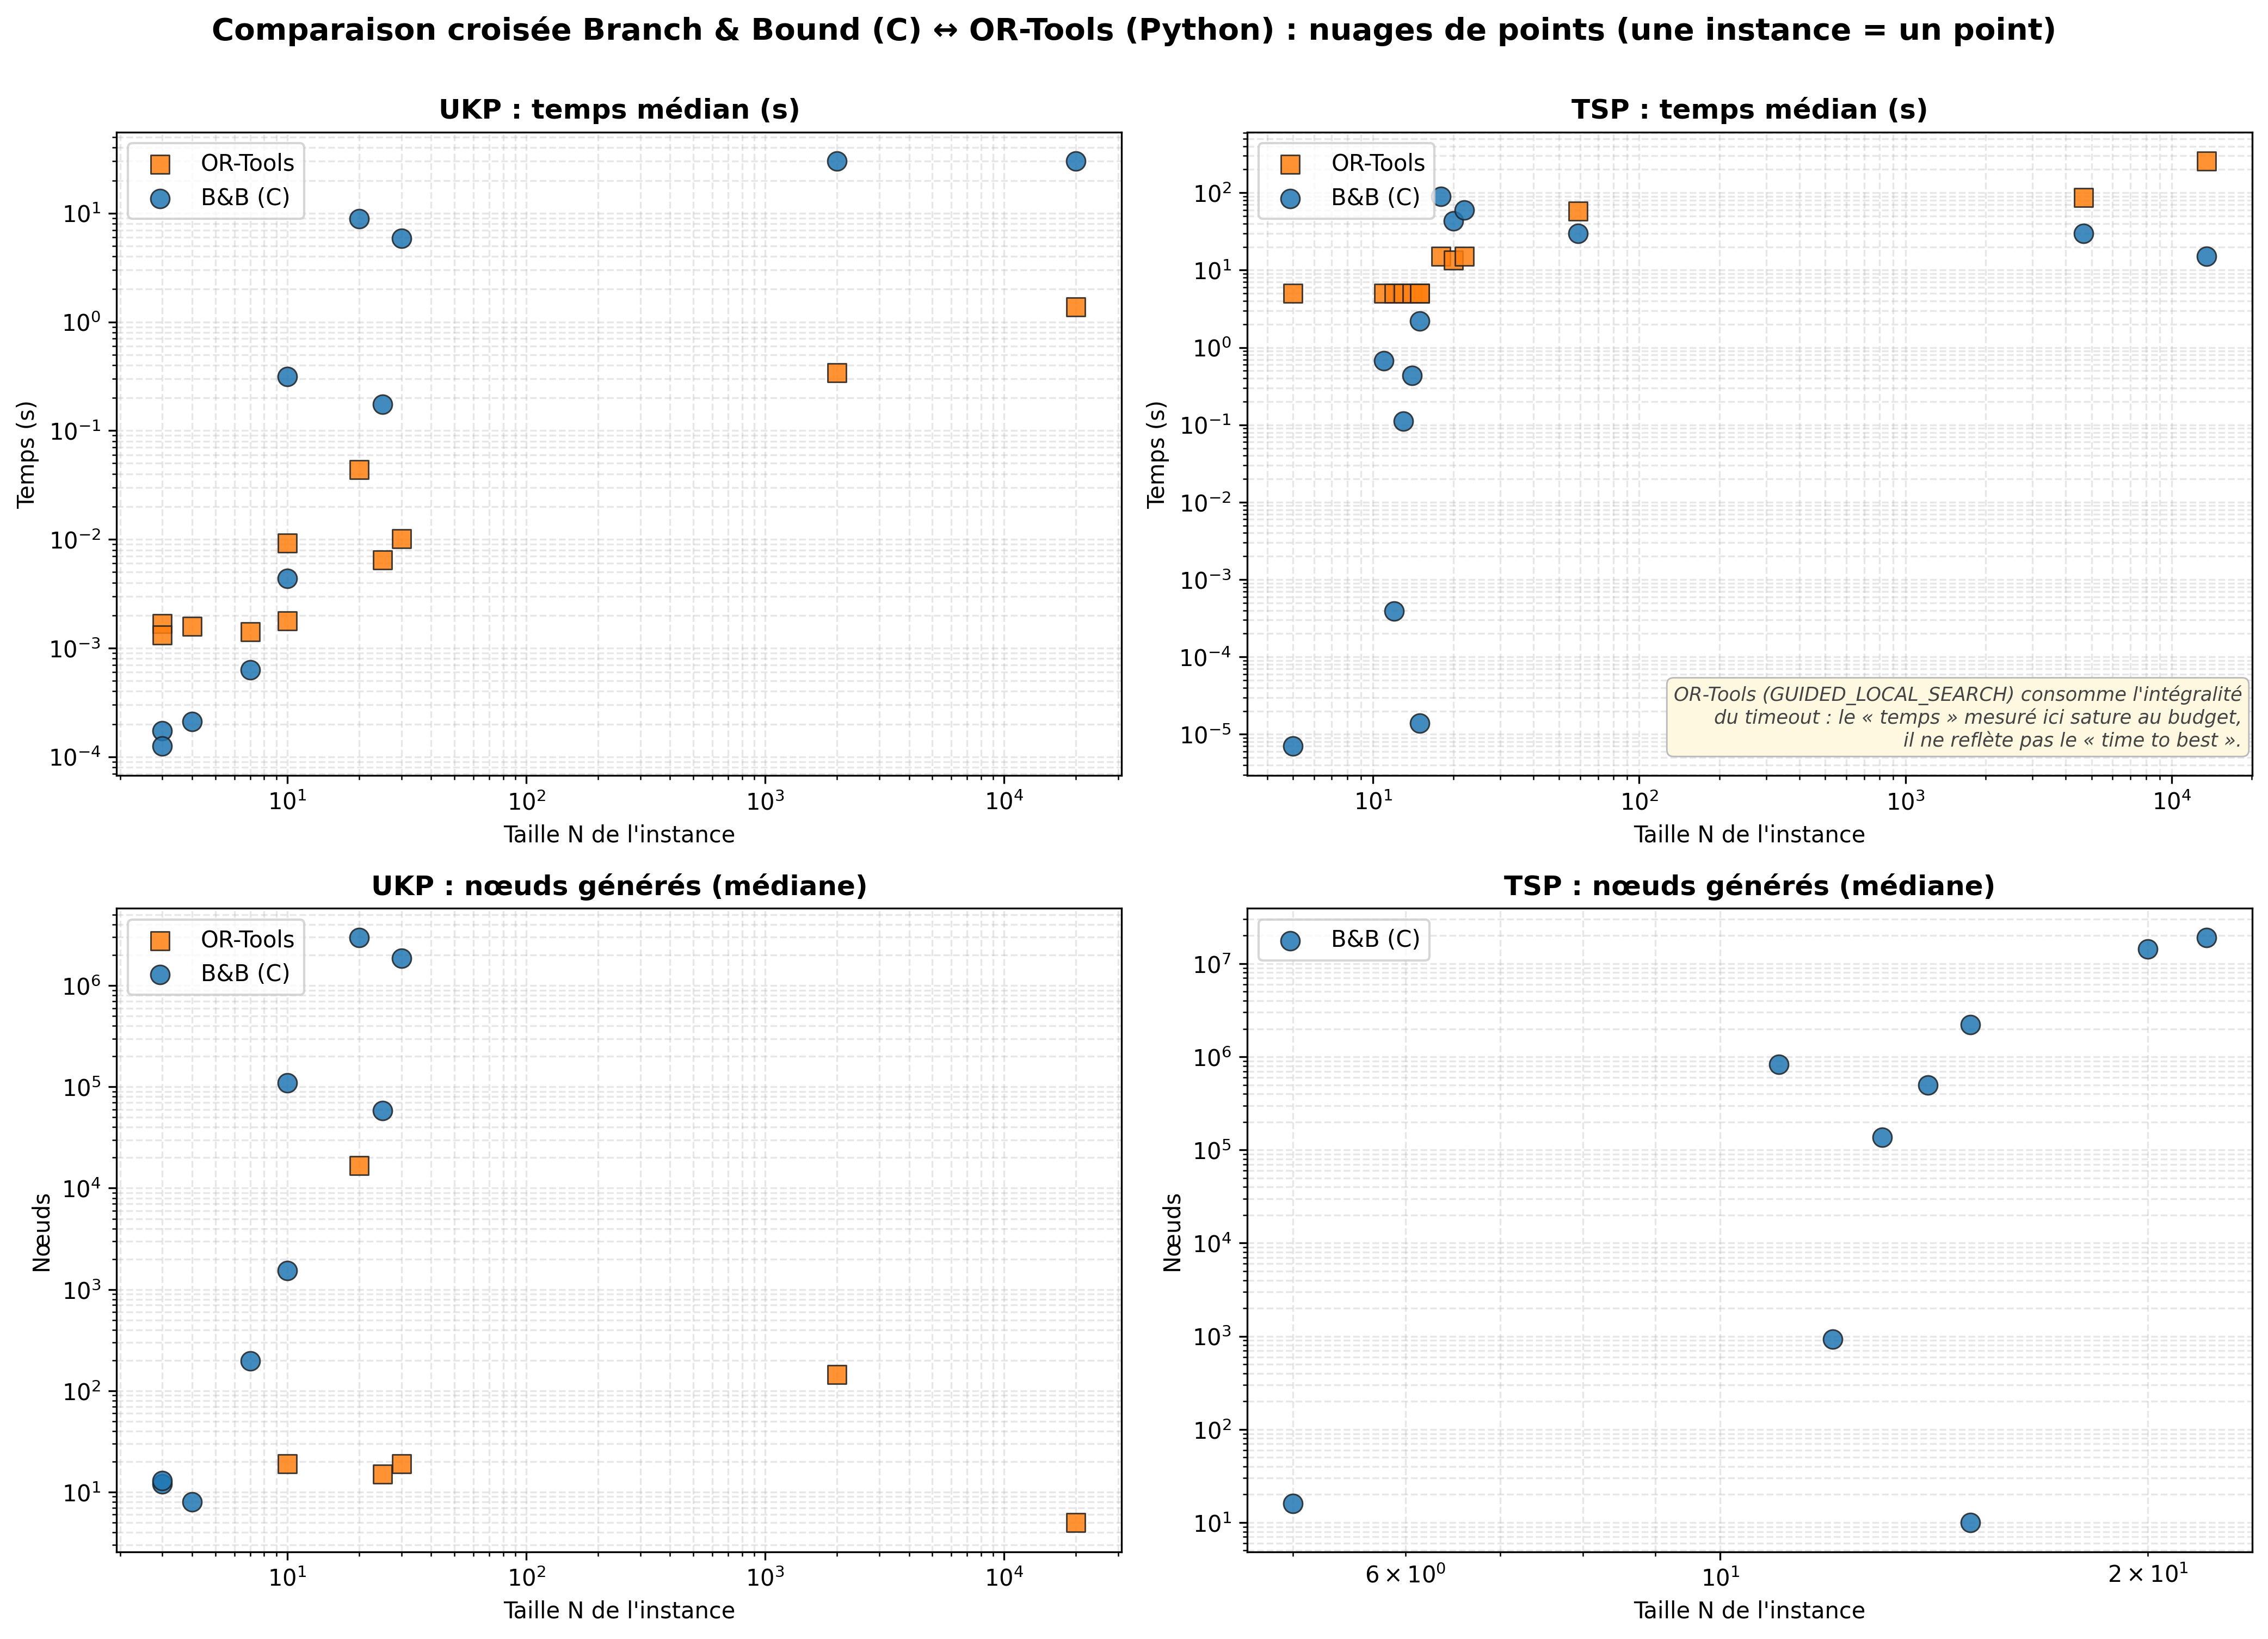
\includegraphics[width=0.92\textwidth]{../Resultats/benchmarks_pousses/panneau_principal.png}
\caption{Comparaison croisée Branch \& Bound (C, en bleu) vs OR-Tools (Python, en orange). Quatre axes log-log en \emph{nuage de points} (\emph{une instance distincte = un point}, médiane des répétitions)~: temps (haut) et nœuds générés (bas), pour UKP (gauche) et TSP (droite). La dispersion verticale du B\&B en UKP révèle la sensibilité au gap LP plutôt qu'à $n$ seul. Un encart explicite sur les sous-figures TSP rappelle qu'OR-Tools (GUIDED\_LOCAL\_SEARCH) consomme \emph{intégralement} son budget temps~: le « temps » mesuré sature au timeout et ne reflète pas le « time to best ».}
\label{fig:panneau}
\end{figure}

\subsection{Variabilité et reproductibilité}

Nous exécutons chaque instance plusieurs fois pour vérifier la stabilité des mesures. La figure~\ref{fig:boxplots} montre les boxplots correspondants. Le B\&B en C est déterministe et présente une dispersion négligeable (boîtes resserrées). OR-Tools côté TSP affiche au contraire des boîtes dégénérées. Toutes les exécutions tombent à la valeur du timeout car GUIDED\_LOCAL\_SEARCH consomme tout le budget temps. Un encart sur la figure documente cette caractéristique pour éviter une interprétation erronée.

\begin{figure}[!htbp]
\centering
\begin{subfigure}[t]{0.49\textwidth}
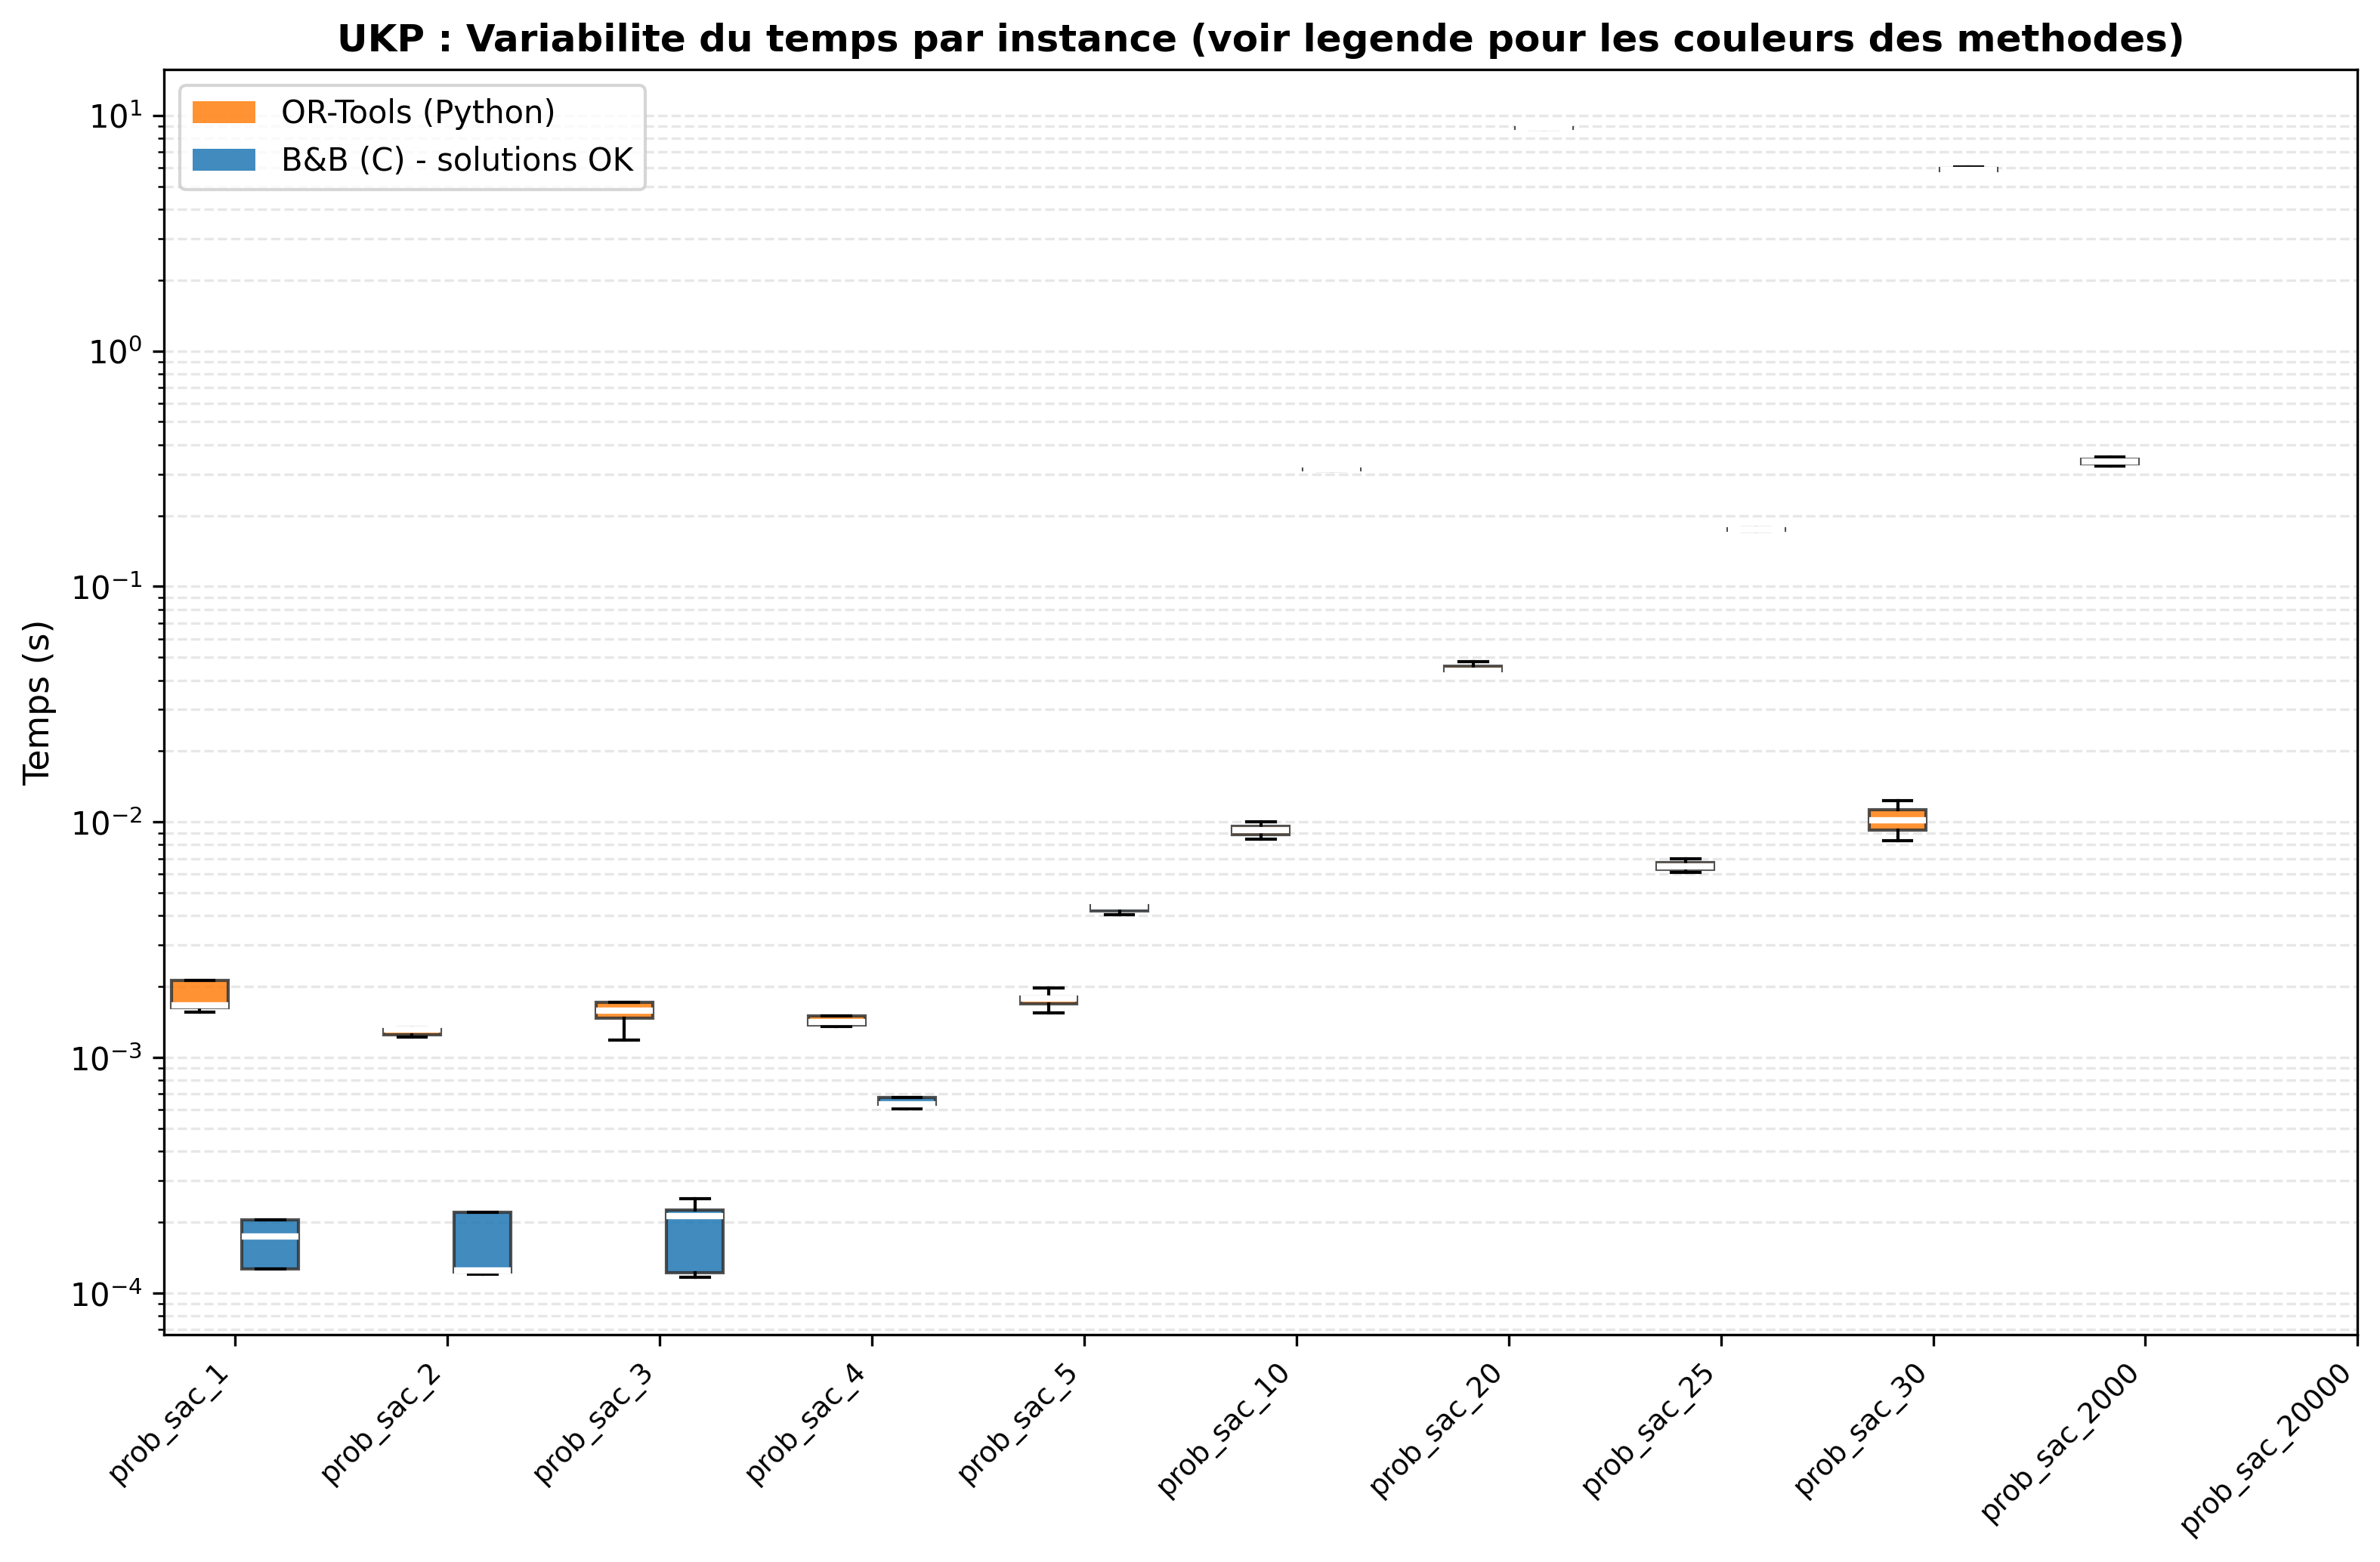
\includegraphics[width=\textwidth]{../Resultats/benchmarks_pousses/boxplot_temps_ukp.png}
\caption{UKP, variabilité par instance}
\end{subfigure}
\hfill
\begin{subfigure}[t]{0.49\textwidth}
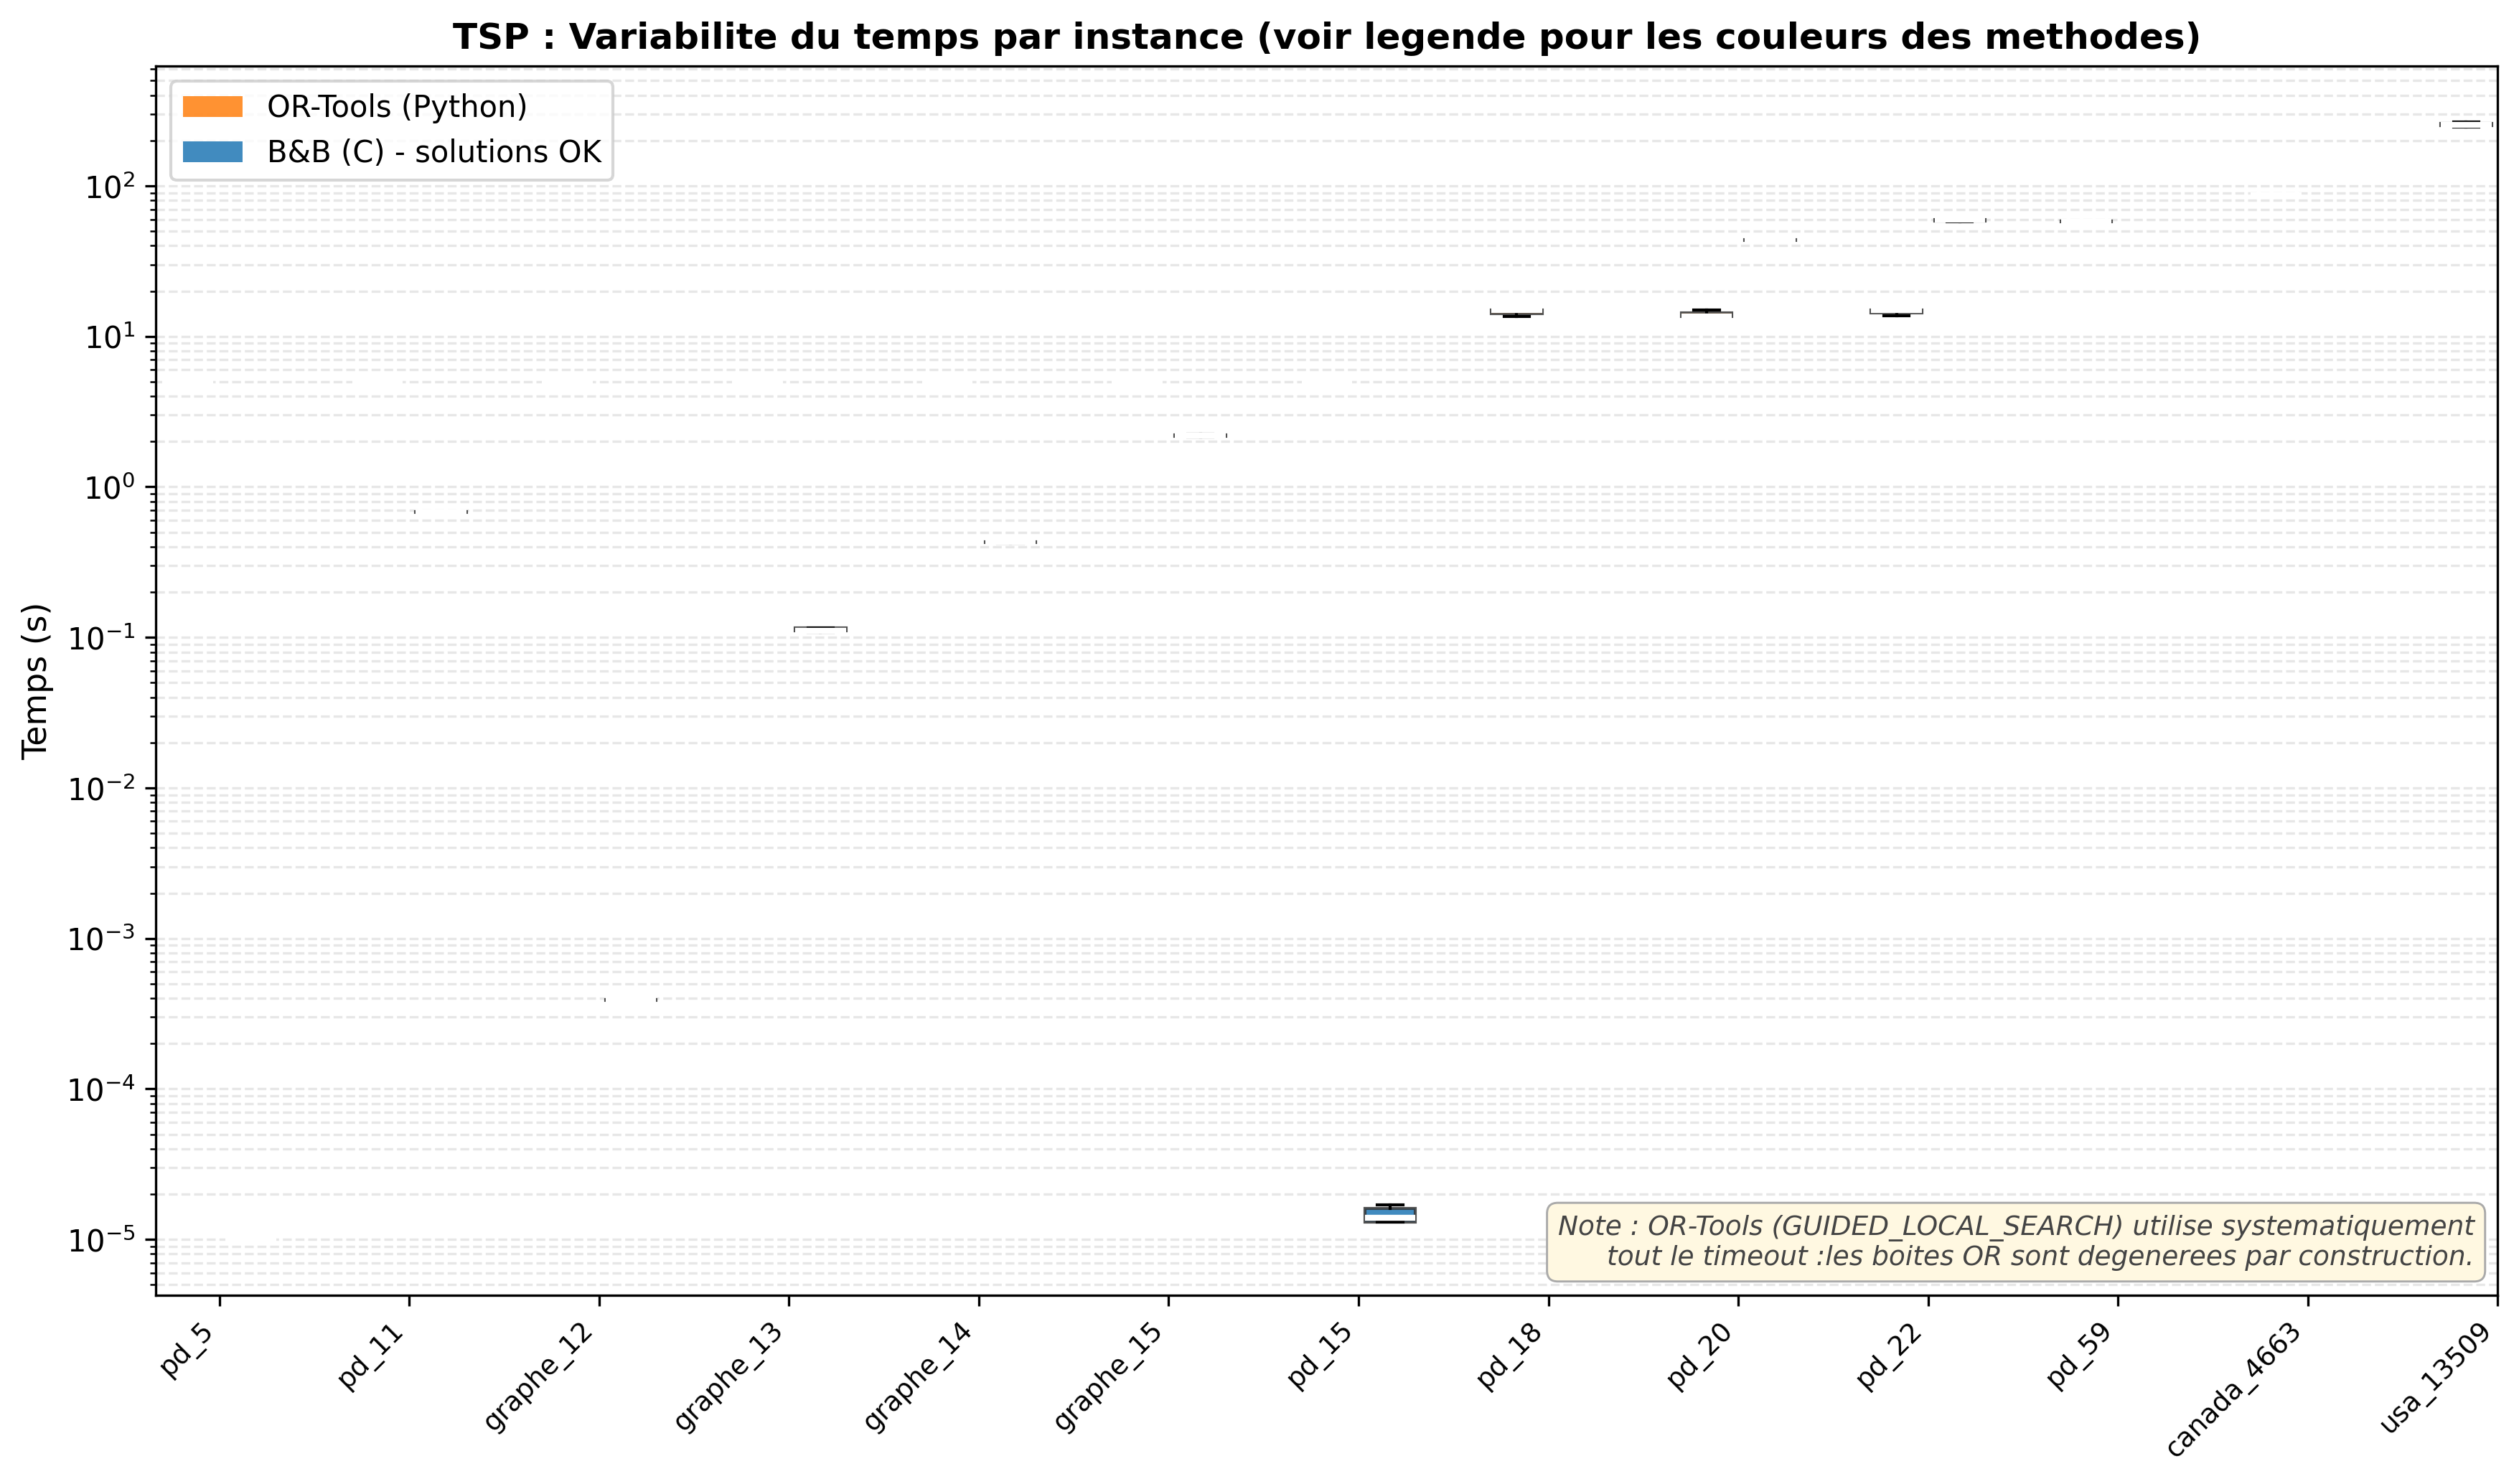
\includegraphics[width=\textwidth]{../Resultats/benchmarks_pousses/boxplot_temps_tsp.png}
\caption{TSP, variabilité par instance}
\end{subfigure}
\caption{Boxplots des temps d'exécution. Le B\&B (en bleu) est stable (déterministe). Côté TSP, OR-Tools (en orange) consomme la totalité du timeout via GUIDED\_LOCAL\_SEARCH. La métrique «~temps~» seule devient peu informative pour cette méthode (point souligné en encart sur la figure).}
\label{fig:boxplots}
\end{figure}

\subsection{Scaling avec barres d'erreur min/max}

La figure~\ref{fig:scaling} trace le temps médian en fonction de la taille de l'instance, avec les bornes min/max en barres d'erreur. Nous étiquetons chaque point par le nom de l'instance. Cela distingue les cas \texttt{prob\_sac\_5} et \texttt{prob\_sac\_10} ($n=10$ identique, capacités très différentes). Cette représentation met en évidence la non-monotonie du B\&B en UKP et l'effet du gap LP discuté plus haut.

\begin{figure}[!htbp]
\centering
\begin{subfigure}[t]{0.49\textwidth}
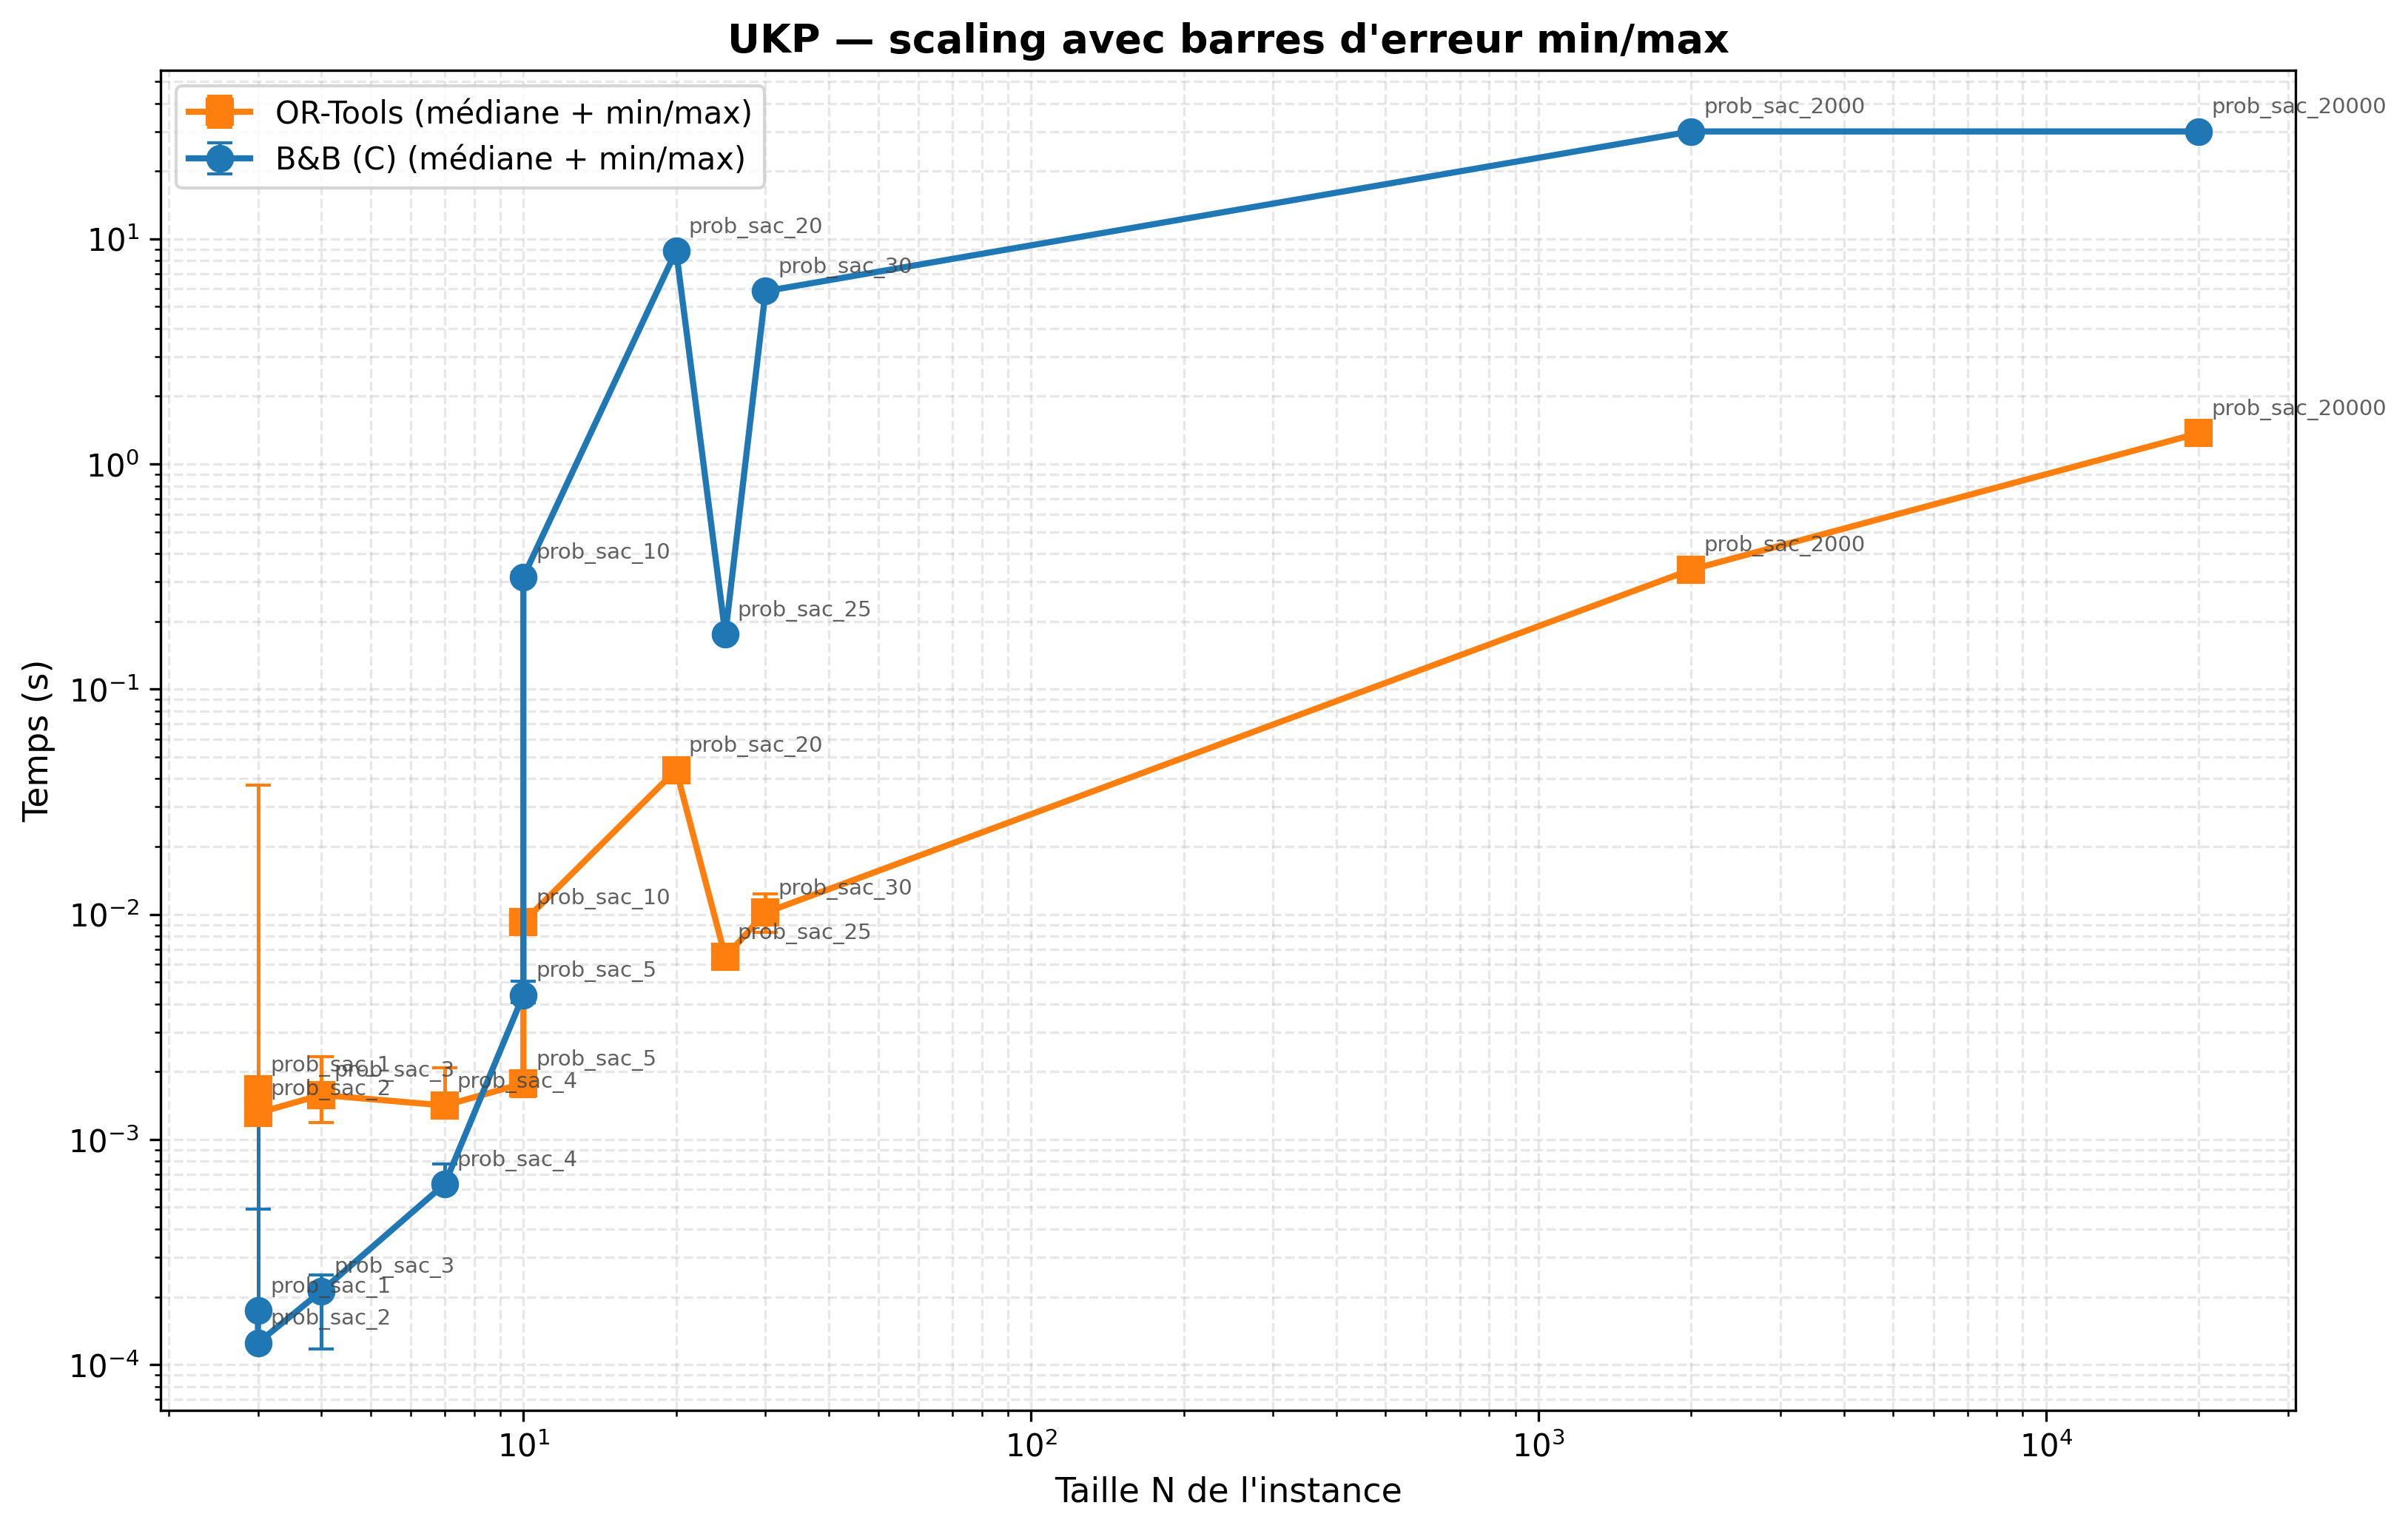
\includegraphics[width=\textwidth]{../Resultats/benchmarks_pousses/scaling_ukp.png}
\caption{UKP}
\end{subfigure}
\hfill
\begin{subfigure}[t]{0.49\textwidth}
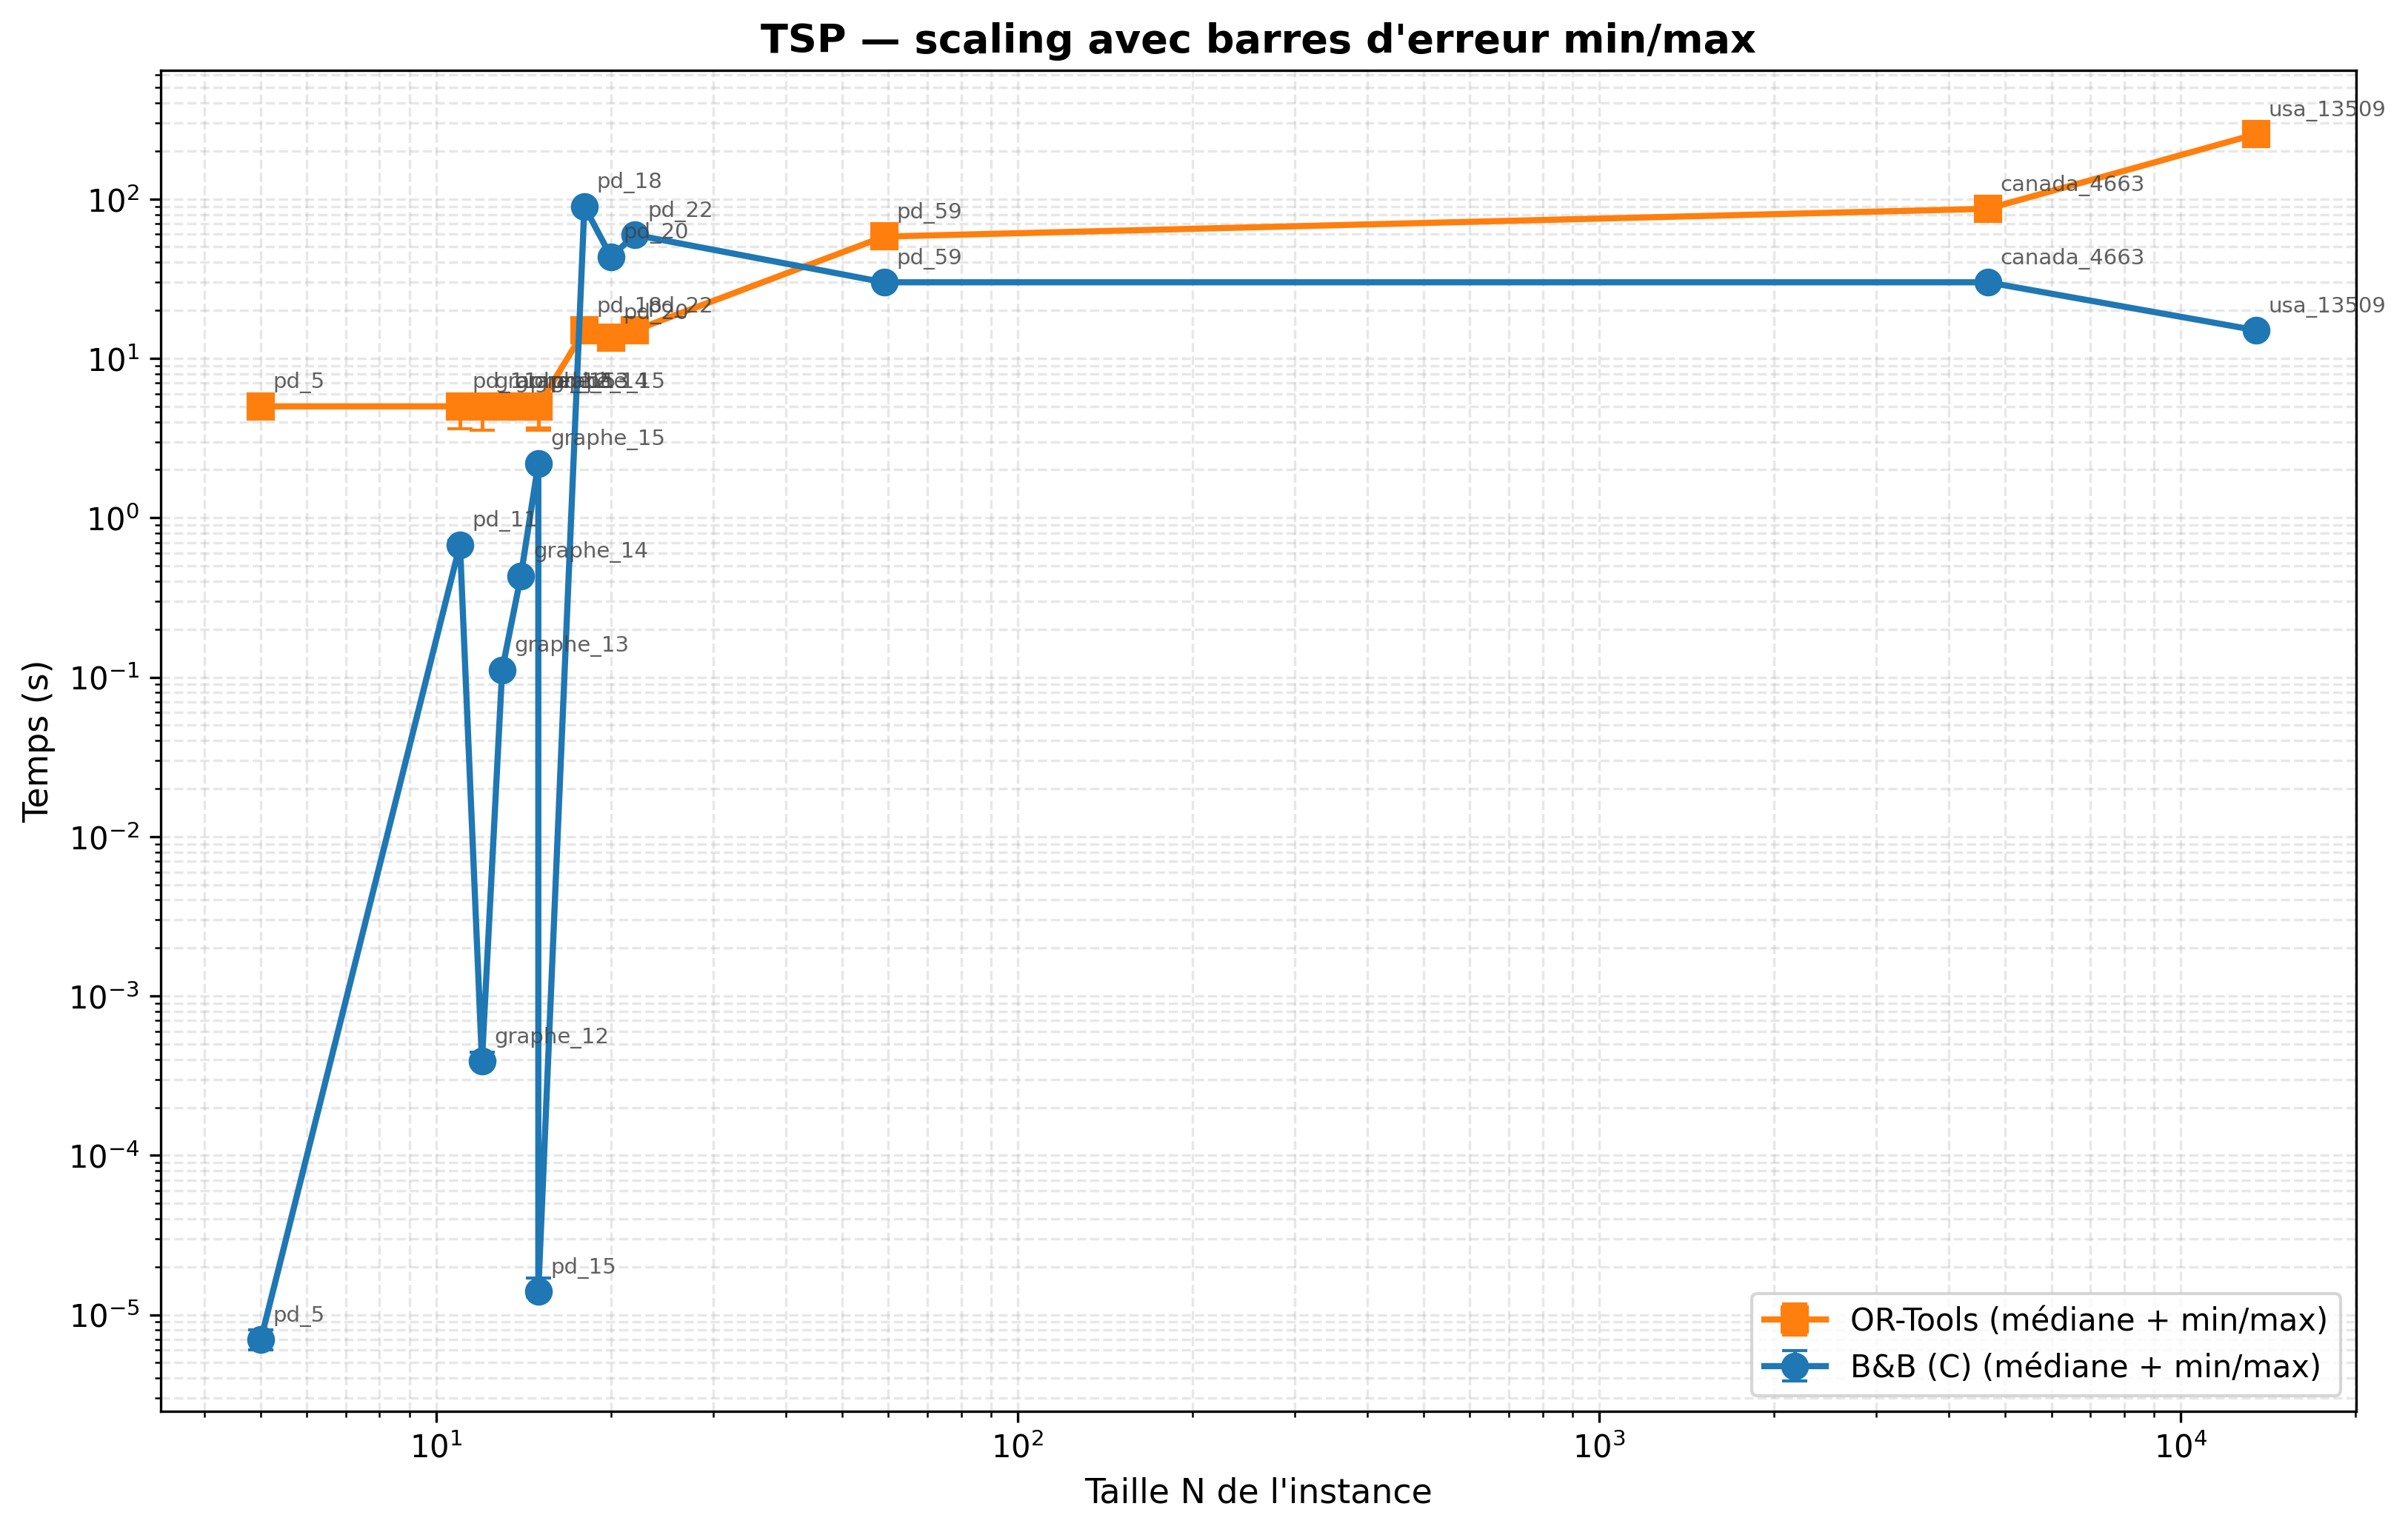
\includegraphics[width=\textwidth]{../Resultats/benchmarks_pousses/scaling_tsp.png}
\caption{TSP}
\end{subfigure}
\caption{Courbes de scaling avec étiquettes d'instance. Pour l'UKP, on note que \texttt{prob\_sac\_5} et \texttt{prob\_sac\_10} ont tous deux $n=10$ mais des temps très différents (4~ms vs 350~ms côté BB), ce qui justifie l'étiquetage individuel des points.}
\label{fig:scaling}
\end{figure}

\subsection{Profil de performance Dolan--Moré}

Le profil de performance de Dolan et Moré~\cite{dolan-more-2002} est l'outil de référence pour comparer plusieurs solveurs sur un ensemble d'instances. Pour un facteur $\tau$ donné, il rapporte la \emph{fraction d'instances} qu'une méthode résout dans un facteur $\tau$ du meilleur temps. Une courbe qui plafonne près de 1 plus tôt en abscisse traduit une méthode plus performante. La figure~\ref{fig:profile} en donne la lecture pour notre benchmark.

\begin{figure}[!htbp]
\centering
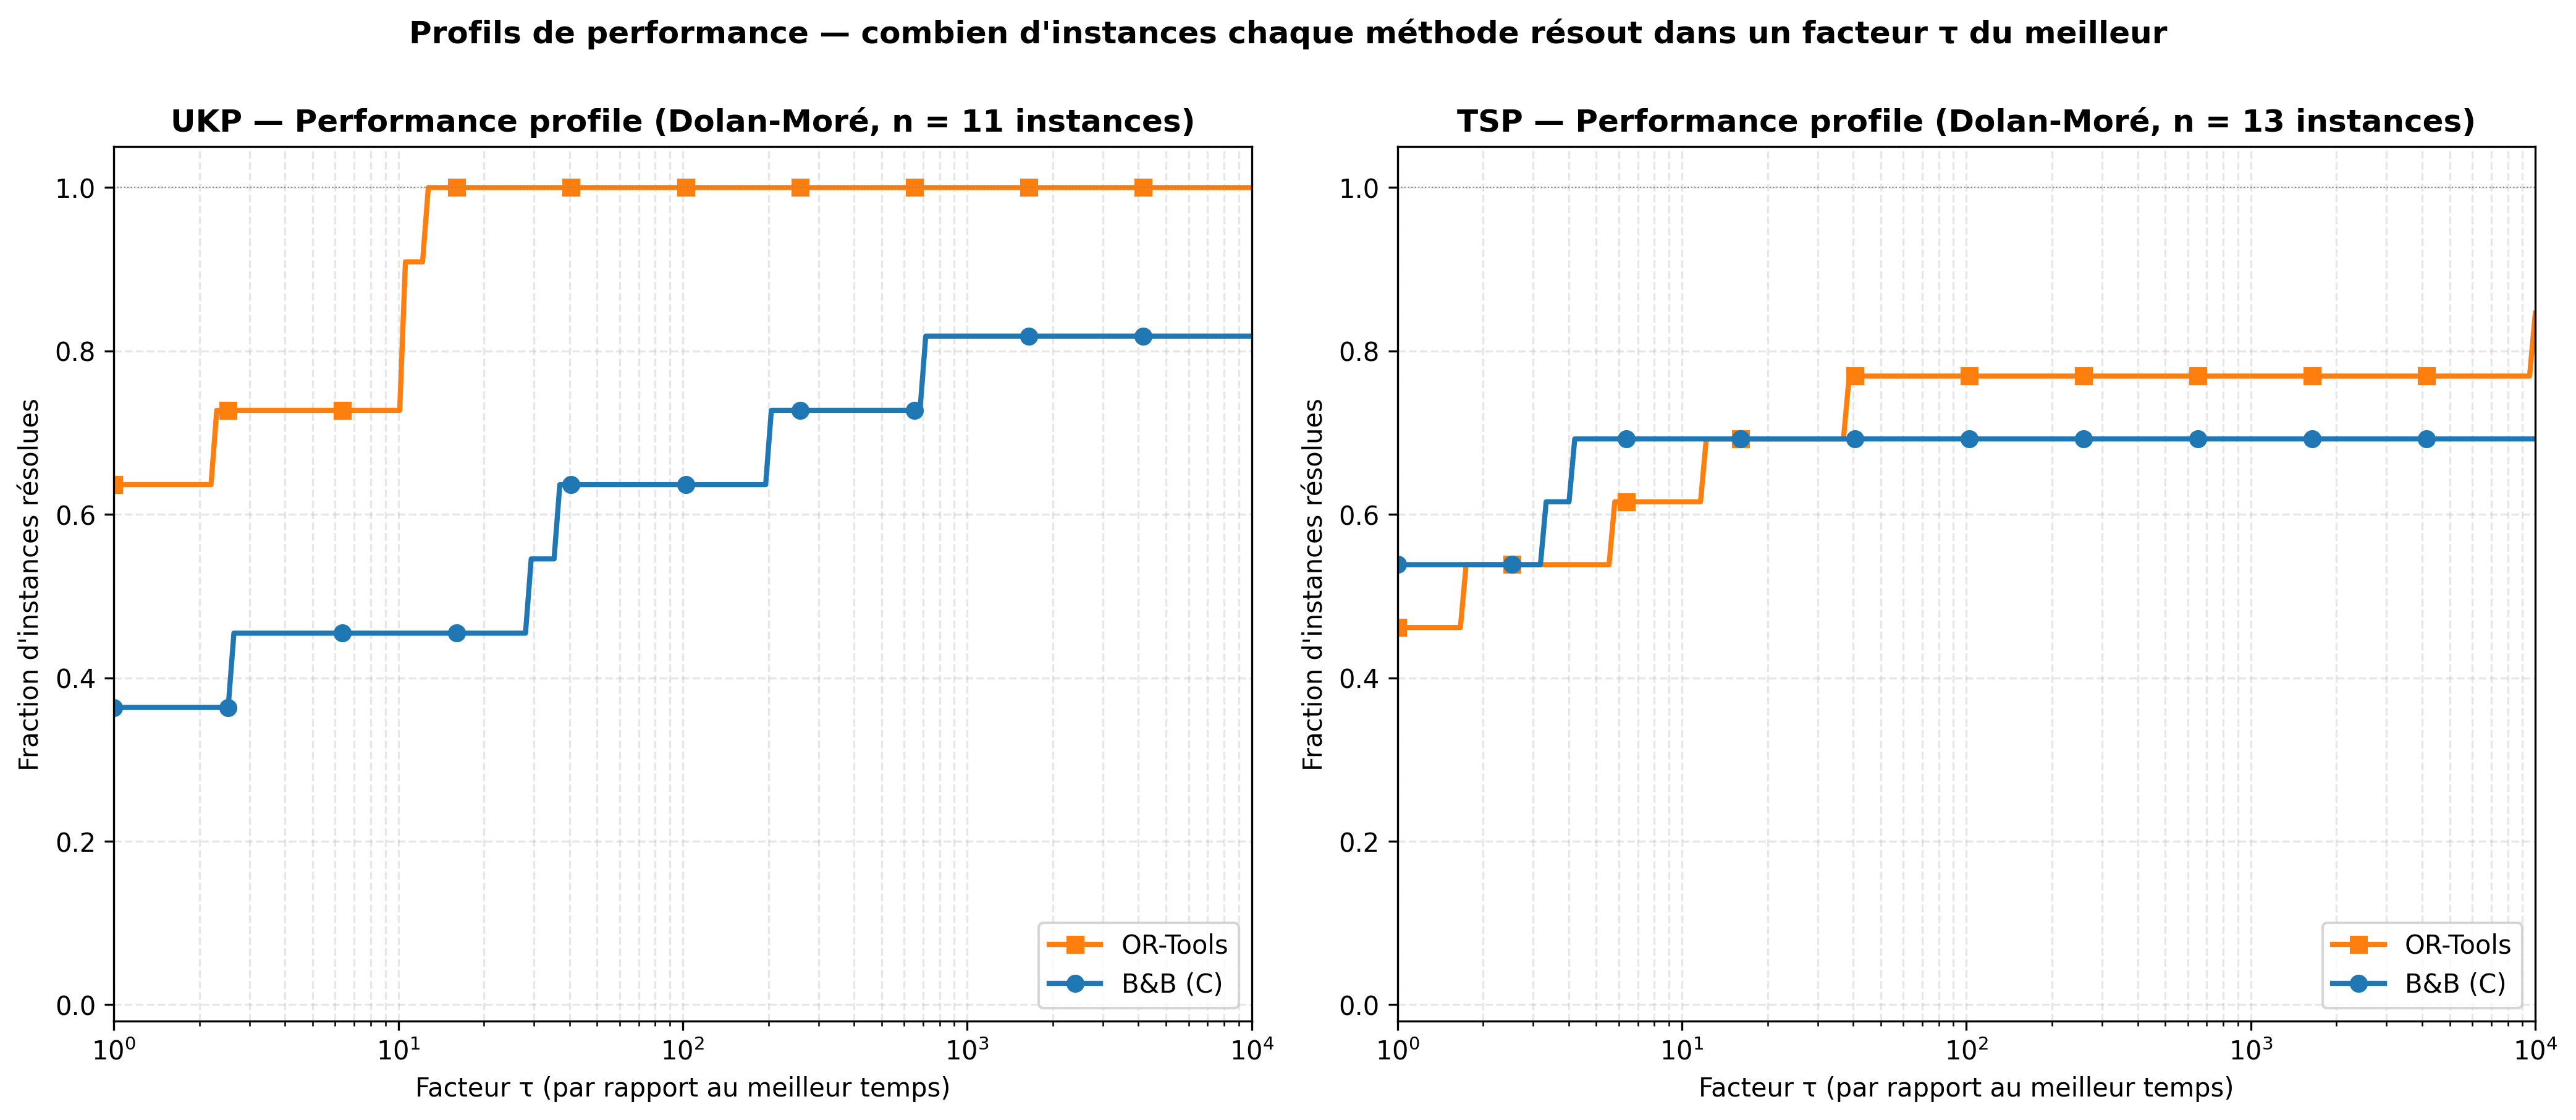
\includegraphics[width=0.92\textwidth]{../Resultats/benchmarks_pousses/performance_profile.png}
\caption{Profil de performance Dolan--Moré. Pour chaque méthode, abscisse $\tau$ = facteur d'écart au meilleur temps, ordonnée = fraction d'instances résolues dans ce facteur. Pour l'UKP (gauche), OR-Tools domine~: il est le plus rapide sur 62~\% des instances dès $\tau=1$ et atteint 100~\% à $\tau \approx 100$. Pour le TSP (droite), B\&B et OR-Tools sont quasiment équivalents au-delà de $\tau \approx 10$, avec une légère avance pour OR-Tools (plus d'instances couvertes au total).}
\label{fig:profile}
\end{figure}

\subsection{Qualité comparée des solutions}

Au-delà du temps, la qualité des solutions reste un critère décisif. La figure~\ref{fig:qualite} affiche, pour chaque instance, le ratio entre la valeur du B\&B et celle d'OR-Tools. Pour l'UKP (maximisation), un ratio supérieur à 1 (en vert) signale une supériorité du B\&B. Pour le TSP (minimisation), un ratio inférieur à 1 indiquerait l'avantage du B\&B en longueur de tour. Toutes les valeurs ici sont à 1. Les deux méthodes convergent donc vers la même solution sur le domaine commun.

\begin{figure}[!htbp]
\centering
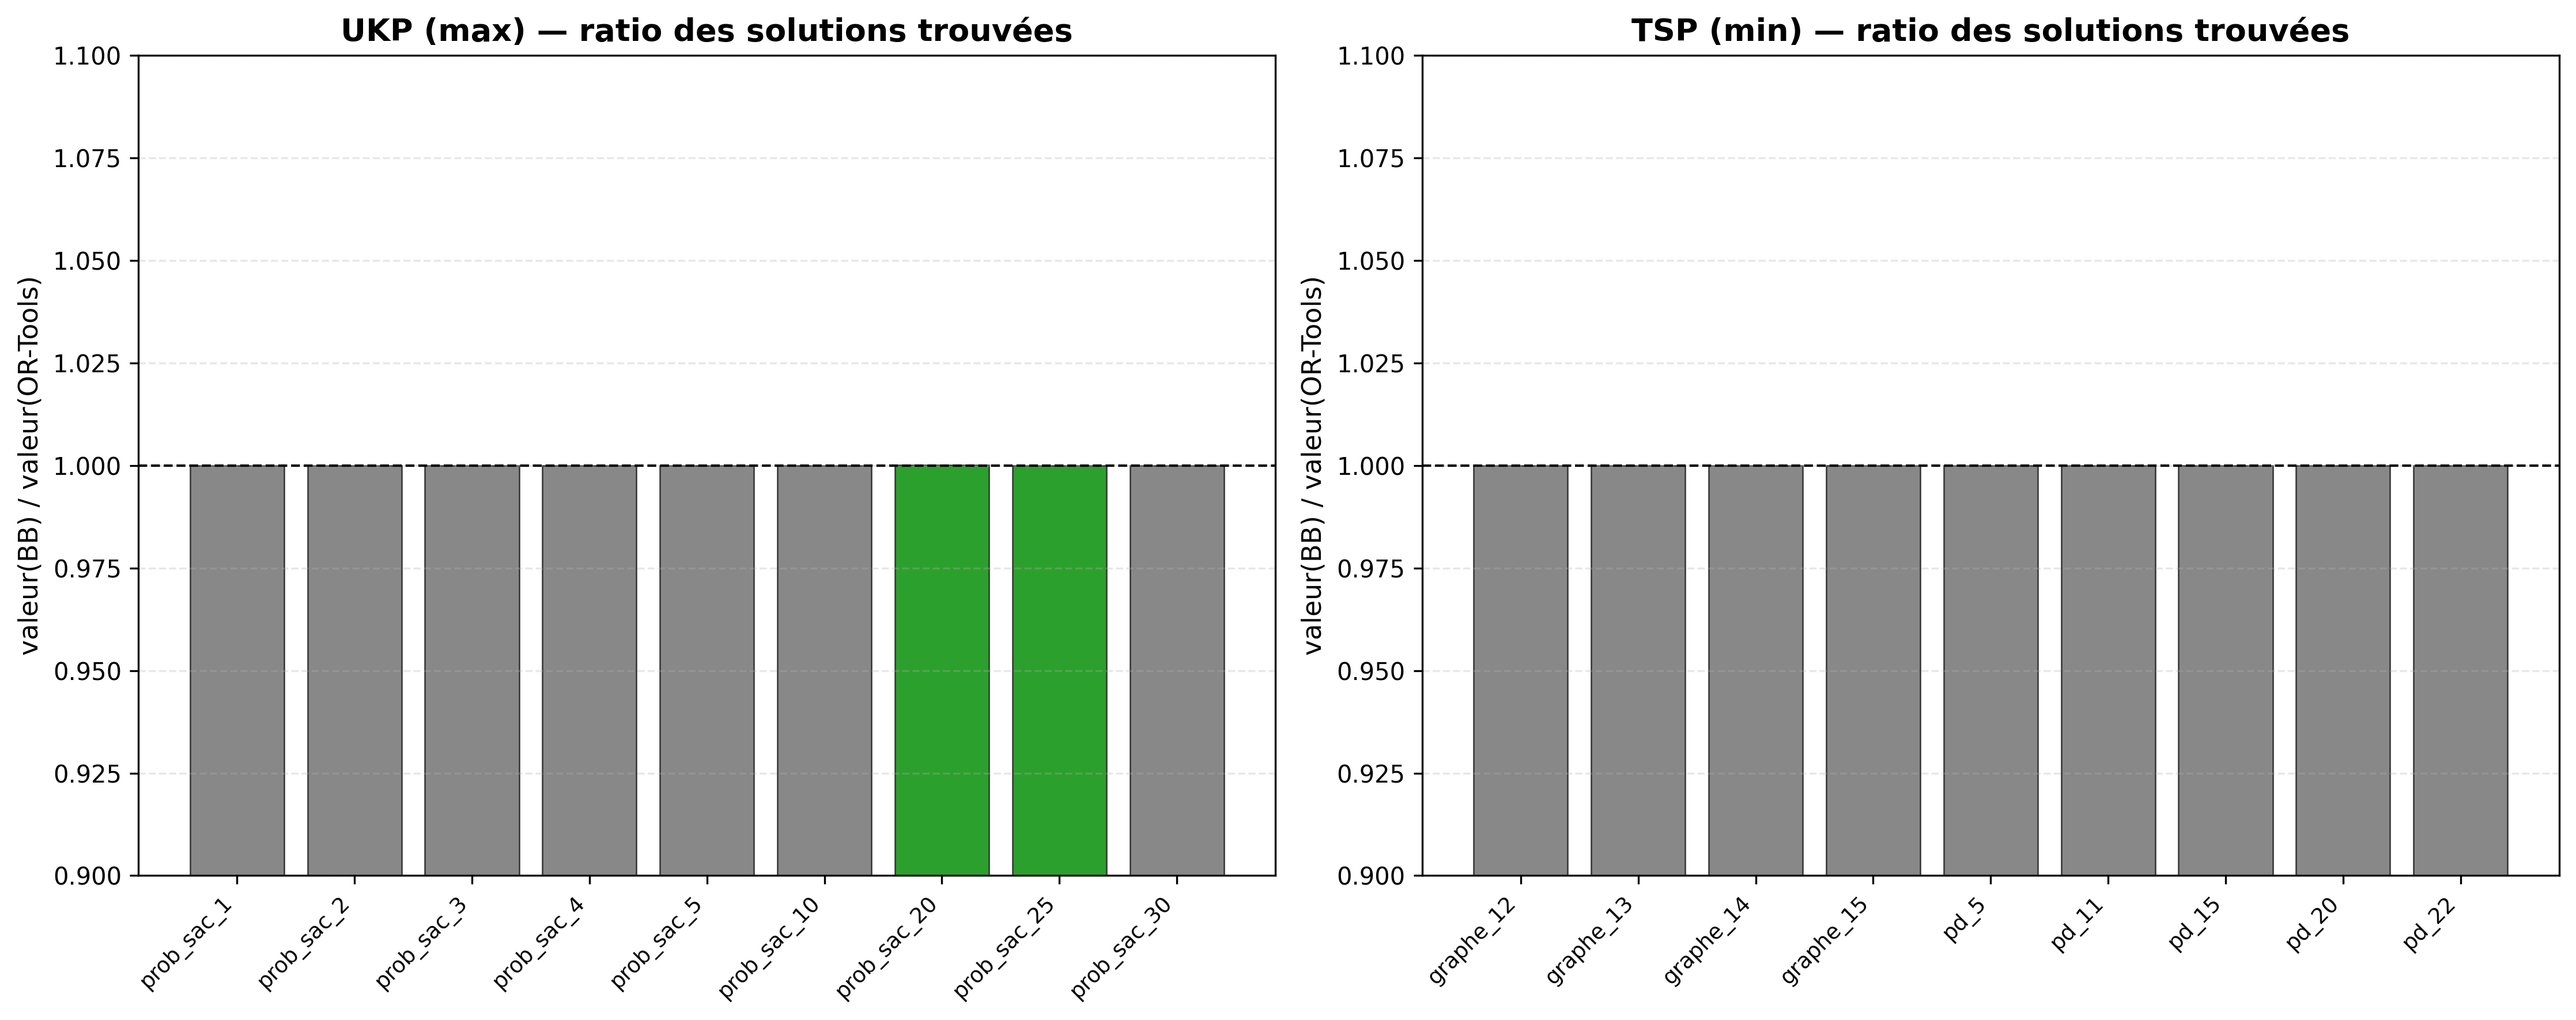
\includegraphics[width=0.92\textwidth]{../Resultats/benchmarks_pousses/qualite_relative.png}
\caption{Ratio valeur(B\&B) / valeur(OR-Tools) par instance. Côté UKP, deux barres vertes signalent une supériorité du B\&B sur \texttt{prob\_sac\_20} (125\,950 vs 125\,942) et \texttt{prob\_sac\_25} (285\,935 vs 285\,934). Côté TSP, toutes les longueurs concordent à l'unité près sur le domaine commun.}
\label{fig:qualite}
\end{figure}

% =============================================================================
\section{Anomalies détectées et vérifications croisées}
\label{sec:anomalies}
% =============================================================================

L'audit qualité a révélé deux instances pour lesquelles OR-Tools renvoie une solution sous-optimale tout en affichant le statut \texttt{OPTIMAL}. Nous certifions cette discordance par programmation dynamique (oracle indépendant)~:

\begin{table}[!htbp]
\centering
\small
\setlength{\tabcolsep}{8pt}
\begin{tabular}{lrrrrr}
\toprule
\textbf{Instance} & \textbf{DP (oracle)} & \textbf{B\&B (C)} & \textbf{OR-Tools (CBC)} & \textbf{Écart CBC} & \textbf{Gap LP--INT} \\
\midrule
\texttt{prob\_sac\_20} & \textbf{125\,950} & \textbf{125\,950}~$\checkmark$ & 125\,942 & $-8$ & $0{,}0023~\%$ \\
\texttt{prob\_sac\_25} & \textbf{285\,935} & \textbf{285\,935}~$\checkmark$ & 285\,934 & $-1$ & $0{,}0004~\%$ \\
\bottomrule
\end{tabular}
\caption{Anomalies CBC validées par DP (oracle indépendant).}
\label{tab:anomalies}
\end{table}

Nous avons d'abord cherché si d'autres solveurs corrigeaient le problème. SCIP~\cite{scip} (\texttt{pywraplp.Solver.CreateSolver("SCIP")}) et BOP renvoient d'autres valeurs sous-optimales, encore différentes ($125\,944$ et $285\,934$ / $285\,909$). Ces solveurs présentent donc eux aussi une faiblesse sur ces instances. Nous avons ensuite mené une investigation paramétrique de CBC via le script \texttt{scripts/\_diag\_cbc\_params.sh}, qui confronte sept configurations~: défauts, gap nul (\texttt{allowableGap 0} + \texttt{ratioGap 0}), \texttt{integerTolerance 1e-12}, désactivation des heuristiques (\texttt{heuristicsOnOff off}), des coupes (\texttt{cutsOnOff off}), du présolveur (\texttt{preprocess off}), enfin une combinaison «~tout brut~». Les sept configurations produisent le même résultat ($125\,942$ / $285\,934$, mêmes $16\,730$ et $15$~nœuds), accompagné de l'avertissement suivant~:
\begin{lstlisting}[language=, basicstyle=\ttfamily\footnotesize]
W linear_solver.cc:1994] SetSolverSpecificParametersAsString()
  not supported by Cbc 2.10.12
\end{lstlisting}
Le binding \texttt{pywraplp} de la version CBC~2.10.12 fournie par OR-Tools ignore silencieusement tout paramétrage transmis. Resserrer le \texttt{ratioGap} ou désactiver les heuristiques depuis Python devient donc impossible, et les défauts internes de CBC s'appliquent en toutes circonstances.

L'interprétation des chiffres devient alors claire. Le tableau~\ref{tab:anomalies} montre que les deux instances possèdent un gap LP--INT très serré. La borne LP relâchée vaut $125\,952{,}95$ pour \texttt{prob\_sac\_20}, soit $+2{,}95$ au-dessus de l'optimum entier $125\,950$, et $285\,936{,}15$ pour \texttt{prob\_sac\_25}, soit $+1{,}15$ au-dessus de l'optimum entier $285\,935$. CBC s'arrête sur des incumbents à $125\,942$ et $285\,934$, ce qui laisse un gap absolu de $10{,}95$ et $2{,}15$ unités vis-à-vis de la borne LP, soit un gap relatif d'environ $0{,}0087~\%$ et $0{,}00075~\%$. Le solveur juge cette précision suffisante, déclare \texttt{OPTIMAL} et manque l'optimum entier. La situation est aggravée par une dégénérescence numérique~: les items \texttt{x3} (ratio $u/v = 1201/57 \approx 21{,}0702$) et \texttt{x1} (ratio $20165/957 \approx 21{,}0710$) de \texttt{prob\_sac\_25} sont quasi-équivalents au sens du ratio utilité/volume, et CBC privilégie le mauvais. La comparaison item-à-item produite par \texttt{\_diag\_compare\_solutions.sh} éclaire la divergence~: la solution DP utilise $9$ items qui remplissent la capacité ($125\,995 = 125\,995$), tandis que CBC en utilise $10$ et laisse $3$ unités libres. Comme $u_i = v_i - 5$, l'écart vaut $\Delta u = \Delta v - 5\,\Delta k = -3 - 5 = -8$ unités d'utilité, ce qui correspond exactement à l'écart observé.

Notre B\&B maison sort renforcé de cette confrontation. Sur les neuf instances UKP testables par DP (\texttt{prob\_sac\_1..30}), il trouve systématiquement la valeur DP. Côté TSP, les neuf instances sur lesquelles il converge donnent une longueur identique à OR-Tools. L'implémentation est donc validée, ce que résume également la sortie textuelle de l'audit automatique sur le dernier benchmark~:

\begin{lstlisting}[language=, basicstyle=\ttfamily\footnotesize]
=== AUDIT QUALITE ===
  WARN | prob_sac_20: BB=125950 > OR=125942 (CBC sous-optimal)
  WARN | prob_sac_25: BB=285935 > OR=285934 (CBC sous-optimal)

  Verification DP exhaustive (petites UKP):
    OK | prob_sac_1..30 : BB == OR == DP

  Verification TSP cross-methode :
    OK | graphe_12..15, pd_5, pd_11, pd_15, pd_20, pd_22

  Recap : 7 OK, 4 WARNING, 0 ERROR
\end{lstlisting}

% =============================================================================
\section{Difficultés rencontrées et améliorations possibles}
\label{sec:discu}
% =============================================================================

\subsection{Difficultés rencontrées}

La première difficulté concerne la mémoire sur \texttt{usa\_13509}. Précomputer la matrice de distances pour $n = 13\,509$ représente près de 5~Go en Python natif, ce qui dépasse la mémoire vive raisonnable d'une machine étudiante. Le programme bascule donc automatiquement vers un calcul à la volée dès $n > 4\,000$.

Les anomalies numériques de CBC ont constitué le deuxième écueil~: aucun message d'erreur ne signale la sous-optimalité, et seule la confrontation avec la DP (oracle) les a révélées. Notre audit qualité automatique détecte désormais ce type de divergence. L'investigation paramétrique de la section~\ref{sec:anomalies} a établi que le binding \texttt{pywraplp} de CBC~2.10.12 ignore silencieusement \texttt{SetSolverSpecificParametersAsString}, ce qui rend impossible toute correction du gap par défaut depuis Python. Deux contournements existent~: un binding alternatif (\texttt{python-mip}, appel direct au binaire \texttt{cbc}) ou un autre solveur. En l'état, notre Branch \& Bound C reste l'unique recours certifié optimal sur ces deux instances.

La troisième difficulté venait de timeouts initialement inadaptés. Une configuration trop courte de 15~s sur \texttt{tsp\_moyens} avait classé \texttt{pd\_20} et \texttt{pd\_22} comme non convergents à tort. En portant ces timeouts à 90~s, nous avons révélé que ces deux instances convergent en réalité en 40 à 52~s.

Enfin, la réécriture des bornes de boucle de \verb|i < n - 1| en \verb|i + 1 < n| (nécessaire pour faire taire les warnings \verb|-Wstrict-overflow=5| de GCC) a coûté environ 10~\% de performance sur les boucles longues du B\&B TSP, une optimisation que GCC effectuait grâce à l'hypothèse d'absence d'\textit{overflow}. Nous assumons ce compromis en faveur d'un code certifié zéro warning.

\subsection{Améliorations possibles}

Plusieurs pistes d'amélioration se dégagent de ce travail. La première consisterait à implémenter une borne TSP plus serrée via la relaxation lagrangienne de Held et Karp sur l'ACPM, ce qui permettrait d'élargir le domaine de convergence du B\&B au-delà de $n = 22$. Une seconde piste serait la parallélisation des branches de l'arborescence avec OpenMP côté C, particulièrement utile sur les instances UKP $n \approx 30$ où le B\&B peut atteindre plusieurs millions de nœuds. Côté métaheuristique, l'ajout d'un Lin-Kernighan en post-traitement offrirait une alternative à OR-Tools pour le TSP de grande taille. Sur le plan de l'instrumentation, nous pourrions enrichir OR-Tools TSP d'un suivi «~time to best~» via un \texttt{SolutionCollector} attaché au \texttt{RoutingModel}, qui journaliserait le temps de découverte de chaque amélioration. La métrique «~temps total~» actuelle est en effet faussement plate, toujours égale au timeout, car GUIDED\_LOCAL\_SEARCH continue de chercher tant qu'il reste du budget. Enfin, une mesure mémoire propre des sous-processus, via \texttt{/usr/bin/time -v} ou \texttt{psutil} autour des appels au binaire C, permettrait de capturer le RSS pic, aujourd'hui non instrumenté.

% =============================================================================
\appendix
\section{Commandes utiles}

\begin{lstlisting}[language=bash, caption={Compilation et tests rapides}]
# Compilation C (Linux/WSL avec libglpk-dev installe)
cd Separation-Evaluation && make
./bin/solveur --probleme ukp --fichier "../Fichiers tests*/prob_sac_1.txt"

# Installation Python et tests OR-Tools
cd OR-Tools && pip install -r requirements.txt
python main.py --probleme tsp --fichier "../Fichiers tests*/pd_5.tsp" --visu

# Pipeline complet (compile + benchmark + figures)
bash scripts/run_all.sh
bash scripts/run_benchmark_pousse.sh --inclure-grands

# Audit qualite automatique (DP sur petites UKP)
bash scripts/_verif_dp_complete.sh
\end{lstlisting}

\section{Liste des livrables}

Le projet est organisé en plusieurs répertoires. Le répertoire \texttt{Separation-Evaluation/} contient l'application C, soit 9 fichiers entre sources et headers, accompagnés de leur Makefile, d'un README et d'une configuration d'exemple. Le répertoire \texttt{OR-Tools/} regroupe l'application Python avec 8 modules, un fichier \texttt{requirements.txt}, un README et une configuration d'exemple. Les résultats des benchmarks figurent dans \texttt{Resultats/benchmarks\_pousses/}, qui rassemble 4 CSV (bruts et agrégés), 7 figures PNG à 300~dpi et un fichier \texttt{ANALYSE.md}. Les visualisations individuelles, soit 9 tours TSP et 7 sacs UKP en haute résolution, se trouvent dans \texttt{Resultats/visualisations/}. Le déploiement HPC est documenté dans \texttt{Romeo/} avec son job SLURM, ses scripts \texttt{rsync} et un README dédié. Enfin, le répertoire \texttt{scripts/} regroupe le pipeline automatisé via \texttt{run\_all.sh}, \texttt{run\_benchmark\_pousse.sh} et \texttt{make\_plots.py}.

% =============================================================================
\section*{Références}
\addcontentsline{toc}{section}{Références}
% =============================================================================

\begin{thebibliography}{99}
\setlength{\itemsep}{0.2em}

\bibitem{dolan-more-2002}
E.~D. \textsc{Dolan} et J.~J. \textsc{Moré},
\textit{Benchmarking optimization software with performance profiles},
Mathematical Programming, vol.~91, n\textsuperscript{o}~2, p.~201--213, 2002.
\href{https://doi.org/10.1007/s101070100263}{doi:10.1007/s101070100263}.

\bibitem{tsplib95}
G.~\textsc{Reinelt},
\textit{TSPLIB, A Traveling Salesman Problem Library},
ORSA Journal on Computing, vol.~3, n\textsuperscript{o}~4, p.~376--384, 1991.
Spécification de format TSPLIB95 (1995) consultée en ligne~:
\href{http://comopt.ifi.uni-heidelberg.de/software/TSPLIB95/}{comopt.ifi.uni-heidelberg.de/software/TSPLIB95/}.

\bibitem{ortools}
L.~\textsc{Perron} et V.~\textsc{Furnon},
\textit{OR-Tools v9.x, Google Operations Research Tools},
Google~LLC, documentation officielle, 2010--2025.
\href{https://developers.google.com/optimization}{developers.google.com/optimization}.

\bibitem{cbc}
J.~\textsc{Forrest} \textit{et~al.},
\textit{COIN-OR Branch-and-Cut Solver (Cbc) version 2.10},
COIN-OR Foundation, 2005--2024.
\href{https://github.com/coin-or/Cbc}{github.com/coin-or/Cbc}.

\bibitem{scip}
K.~\textsc{Bestuzheva} \textit{et~al.},
\textit{The SCIP Optimization Suite 8.0},
ZIB Report 21-41, Zuse Institute Berlin, 2021.
\href{https://www.scipopt.org/}{scipopt.org}.

\bibitem{glpk}
A.~\textsc{Makhorin},
\textit{GLPK, GNU Linear Programming Kit, version 5.0},
Free Software Foundation, 2000--2020.
\href{https://www.gnu.org/software/glpk/}{gnu.org/software/glpk}.

\bibitem{land-doig}
A.~H. \textsc{Land} et A.~G. \textsc{Doig},
\textit{An automatic method of solving discrete programming problems},
Econometrica, vol.~28, n\textsuperscript{o}~3, p.~497--520, 1960.
\href{https://doi.org/10.2307/1910129}{doi:10.2307/1910129}.

\bibitem{kellerer-knapsack}
H.~\textsc{Kellerer}, U.~\textsc{Pferschy} et D.~\textsc{Pisinger},
\textit{Knapsack Problems},
Springer, Berlin, 2004. ISBN~3-540-40286-1.

\bibitem{applegate-tsp}
D.~L. \textsc{Applegate}, R.~E. \textsc{Bixby}, V.~\textsc{Chvátal} et W.~J. \textsc{Cook},
\textit{The Traveling Salesman Problem: A Computational Study},
Princeton University Press, 2006. ISBN~0-691-12993-2.

\bibitem{lin-kernighan}
S.~\textsc{Lin} et B.~W. \textsc{Kernighan},
\textit{An effective heuristic algorithm for the traveling-salesman problem},
Operations Research, vol.~21, n\textsuperscript{o}~2, p.~498--516, 1973.
\href{https://doi.org/10.1287/opre.21.2.498}{doi:10.1287/opre.21.2.498}.

\bibitem{voudouris-gls}
C.~\textsc{Voudouris} et E.~\textsc{Tsang},
\textit{Guided Local Search and its application to the traveling salesman problem},
European Journal of Operational Research, vol.~113, n\textsuperscript{o}~2, p.~469--499, 1999.
\href{https://doi.org/10.1016/S0377-2217(98)00099-X}{doi:10.1016/S0377-2217(98)00099-X}.

\end{thebibliography}

\end{document}
